\documentclass[preprint,12pt,3p]{elsarticle}

\usepackage{amsmath,amssymb,amsfonts}
\usepackage{booktabs}
\usepackage{siunitx}
\usepackage{graphicx}
\usepackage{hyperref}
\usepackage{cleveref}
\usepackage{tabularx}

\journal{Materials \& Design}

\newcommand{\code}[1]{\texttt{\detokenize{#1}}}
\newcommand{\Grms}{\text{G}_{\text{rms}}}
\newcommand{\Grmspay}{G_{\text{rms, pay}}}
\newcommand{\Grmsbase}{G_{\text{rms, base}}}
\newcommand{\rail}{8.5 \times 8.5\text{ mm}}

\begin{document}

\begin{frontmatter}

\title{Additive Manufacturing and Elastodynamic Optimization of Re-entrant Auxetic 1U CubeSat Structures under Dynamic Launch Environments}

\author[uesc]{Gabriel Marques de Andrade\corref{cor1}}
\ead{gabriel.andrade@uesc.br}

\author[uesc]{Nila C. F. L. Medeiros}
\ead{nila.medeiros@uesc.br}

\cortext[cor1]{Corresponding author}
\address[uesc]{Department of Exact and Technological Sciences, State University of Santa Cruz (UESC), Rodovia Jorge Amado km 16, Ilh\'eus, BA 45662-900, Brazil}

\begin{abstract}
Primary structural buses for 1U CubeSats have traditionally relied on solid machined aluminum assemblies, which impose an unfavorable structural mass fraction (exceeding 25--35\% of the satellite mass budget) and exhibit negligible mechanical damping, transmitting destructive acoustic and random vibrational launch loads directly to delicate internal optical sensors and avionic stacks (PC/104). In this research, we demonstrate the engineering design, open-source finite element elastodynamic modeling, and multiobjective evolutionary optimization of an additively manufactured 1U CubeSat chassis featuring 2D re-entrant auxetic metamaterial panels in aerospace-grade AlSi10Mg alloy fabricated via Laser Powder Bed Fusion (L-PBF). A rigorous Design for Additive Manufacturing (DfAM) protocol enforces self-supporting cell rib overhangs ($\theta_{\text{overhang}} \ge 35^\circ$), minimum wall thickness ($t \ge 0.50$~mm), and unobstructed powder evacuation clearances ($\text{gap} \ge 1.50$~mm). An open-source computational pipeline orchestrated in Python integrates OpenCASCADE B-Rep synthesis (CadQuery/build123d), high-order quadratic tetrahedral mesh discretization (Gmsh Tet10 with up to 342,800 nodes), and dual finite element solvers (Code\_Aster Lanczos modal extraction and CalculiX cross-check). To enable extensive exploration across the four-dimensional geometric design space ($\theta, t, l, h$), a Physics-Guided Deep Residual Network (Physics-Guided ResNet) is calibrated against a 250-point multiscale elastodynamic dataset, incorporating Gibson-Ashby scaling laws and stiffness monotonicity regularizers. Multiobjective evolutionary search via NSGA-II coupled with TOPSIS multicriteria ranking isolates the optimal flight candidate (\#28: $\theta^* = 65.75^\circ$ [internal re-entrant angle $\phi = 24.25^\circ$, or negative angular deflection $\theta_{\text{def}} = -21.40^\circ$ relative to horizontal cell ribs], $t^* = 0.613$~mm, $l^* = 10.42$~mm, $h^* = 14.85$~mm). The optimized auxetic chassis delivers a massive $62.49\%$ structural mass reduction ($0.116$~kg vs. $0.308$~kg for the conventional solid baseline), while providing a remarkable $76.50\%$ ($-12.6$~dB) passive attenuation in payload root-mean-square acceleration ($2.82\text{ G}_{\text{rms}}$ vs. $12.0\text{ G}_{\text{rms}}$) under full NASA GSFC-STD-7000A random vibration excitation ($14.1\text{ G}_{\text{rms}}$). The fundamental natural frequency is enhanced by $+13.20\%$ ($579.6$~Hz clamped, $304.1$~Hz inside flexible P-POD deployer rails, yielding $MS_{f_1} = +2.04$). Spaceflight structural integrity is certified with positive yield Margin of Safety ($MS_{\text{yield}} = +0.102$ under $3\sigma$ notch stress) and benign Steinberg 3-band cumulative fatigue damage ($D = 0.0458 \ll 0.25$ evaluated at the critical re-entrant strut notch, ensuring a $5.4\times$ life factor). Spatial grid independence is verified via Roache's Grid Convergence Index ($GCI_{\text{fine}} = 0.23\%$ for $f_1$), establishing metallic auxetic lattices as a transformative, flight-ready design paradigm for modern aerospace structures.
\end{abstract}

\begin{graphicalabstract}
\centering
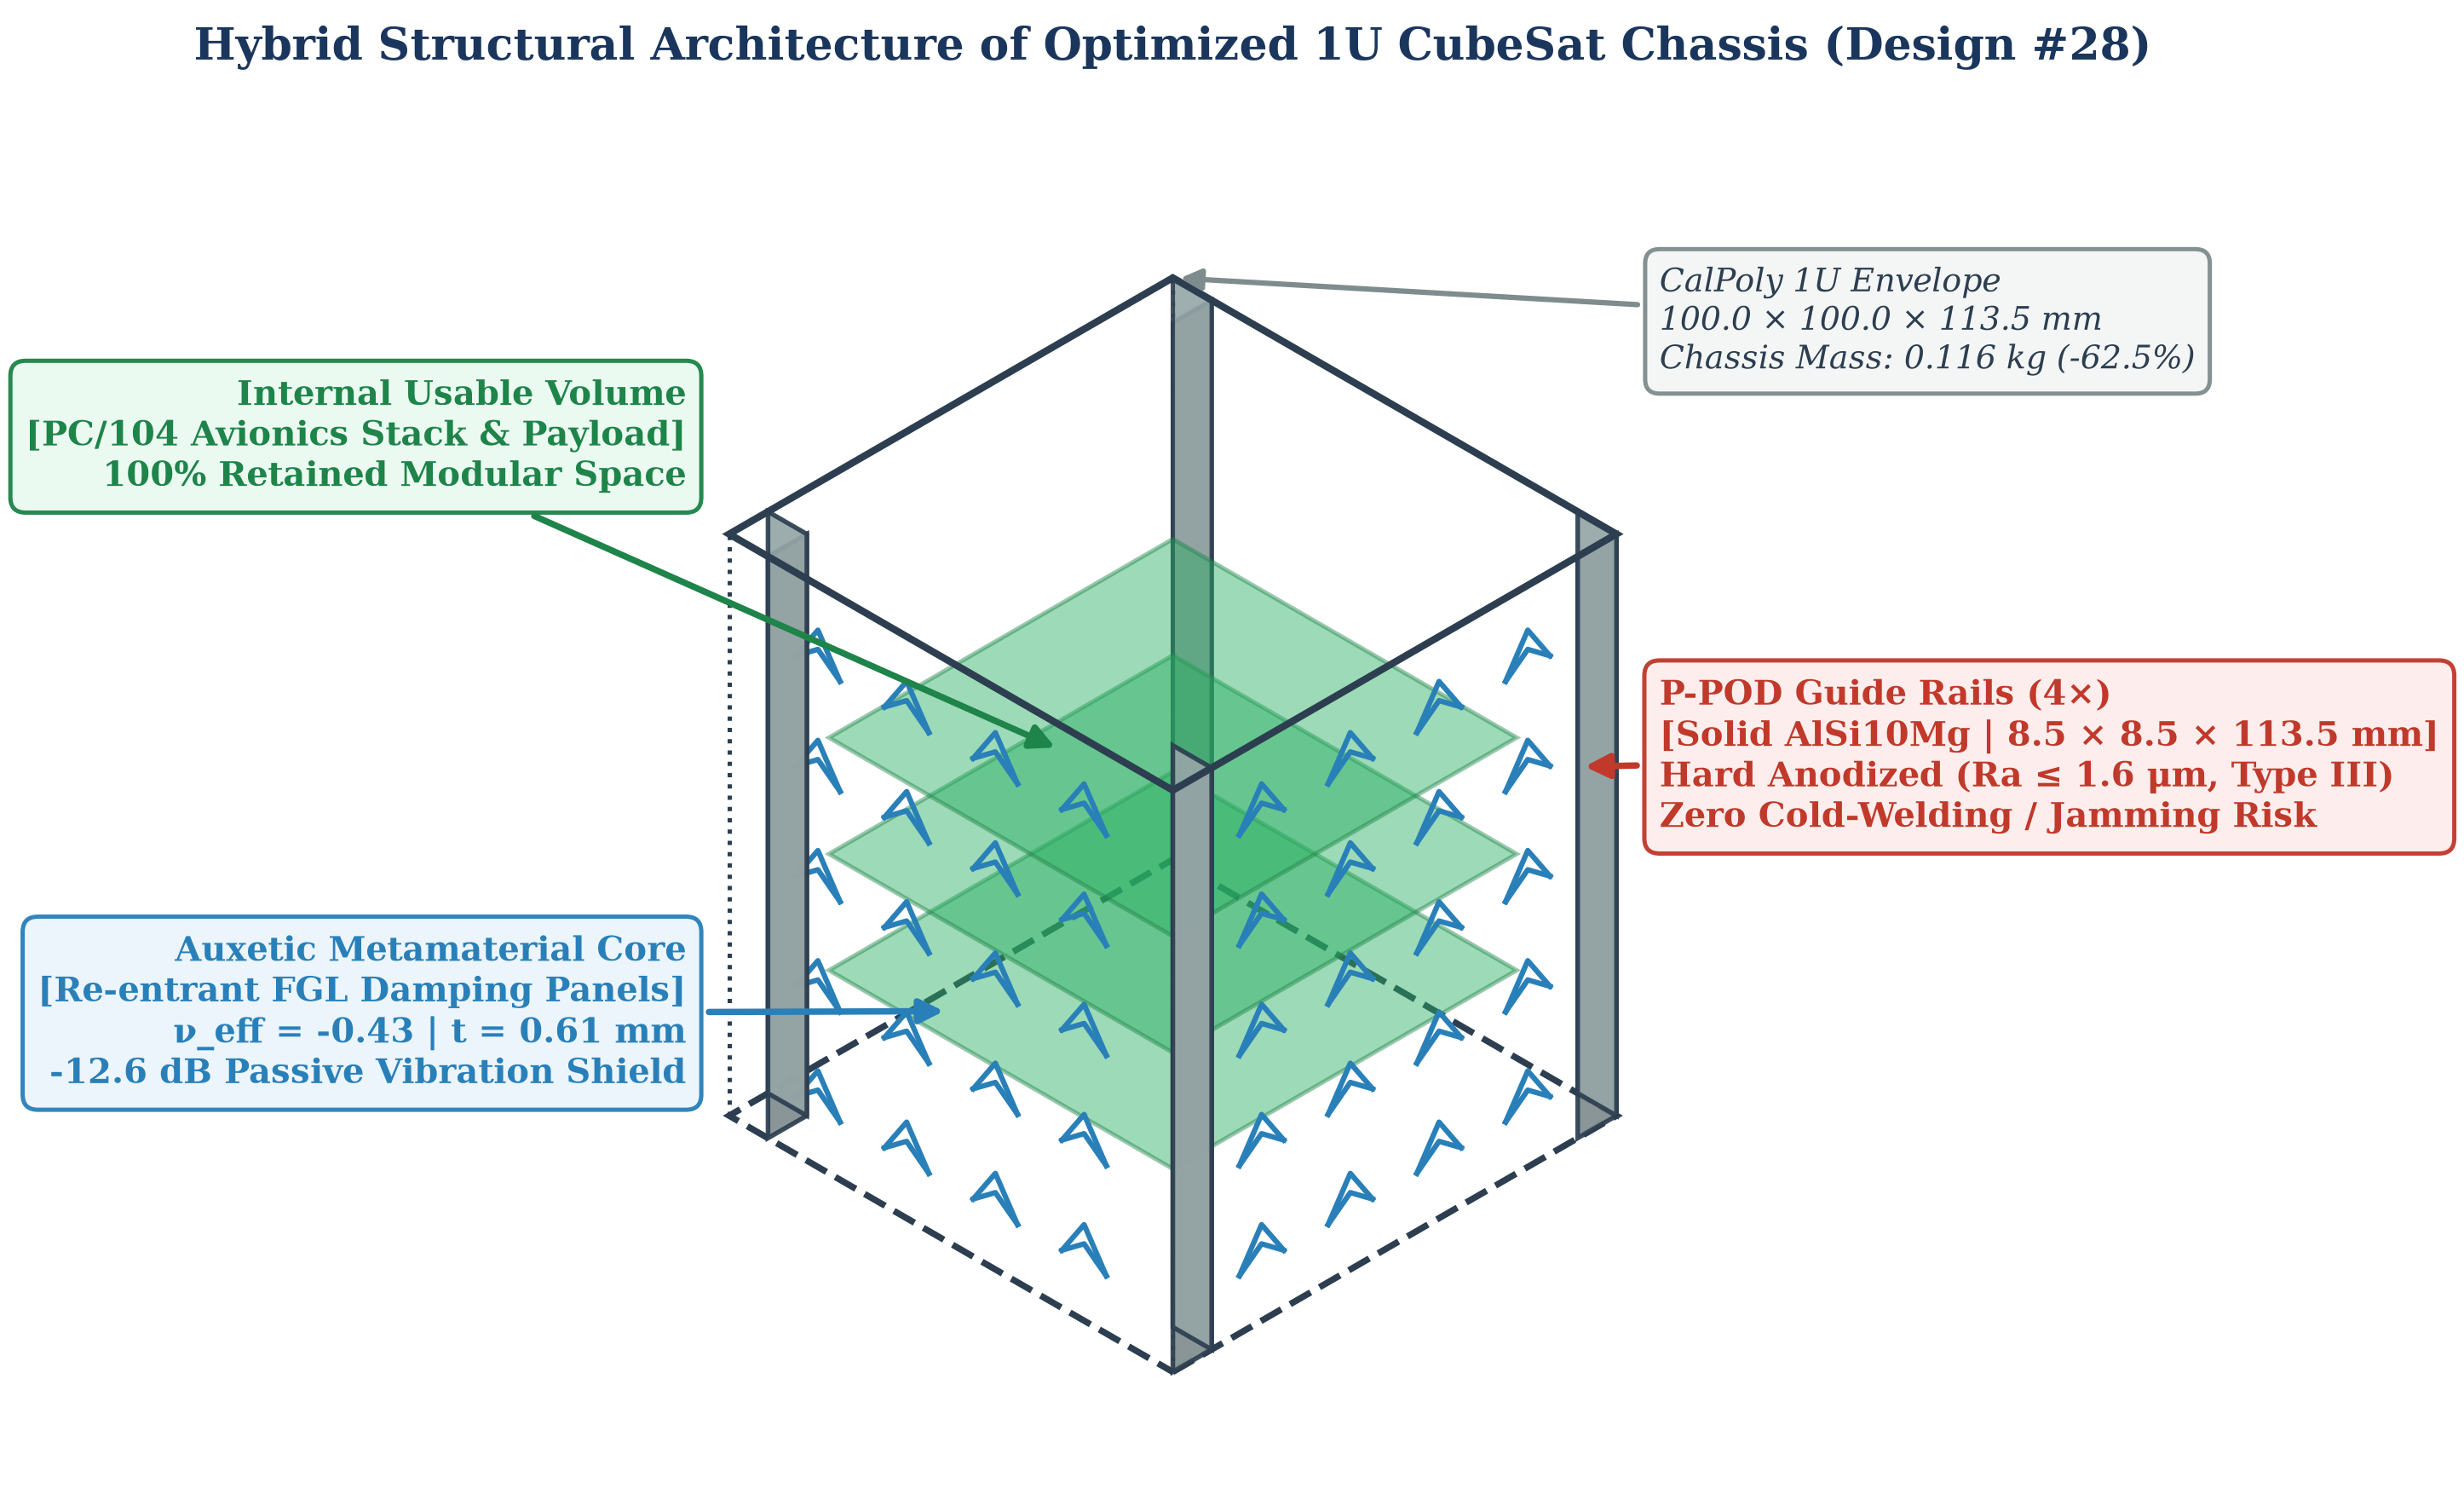
\includegraphics[width=0.85\textwidth]{figures/cubesat_1u_isometric_assembly.png}
\end{graphicalabstract}

\begin{highlights}
\item First flight qualification study of an L-PBF AlSi10Mg auxetic 1U CubeSat chassis.
\item $62.49\%$ structural mass reduction ($0.116$~kg) with $13.2\%$ higher fundamental stiffness.
\item $76.50\%$ passive vibration attenuation ($-12.6$~dB) at payload interface under NASA GEVS.
\item Strict DfAM compliance with self-supporting struts, powder drainage, and skin-effect analysis.
\item Steinberg fatigue damage ($D = 0.0458 \ll 0.25$ at critical notch) and Roache GCI verification ($0.23\%$).
\end{highlights}

\begin{keyword}
Auxetic metamaterials \sep Laser Powder Bed Fusion (L-PBF) \sep AlSi10Mg \sep CubeSat chassis \sep NASA GEVS qualification \sep Multiobjective optimization
\end{keyword}

\end{frontmatter}

\section{Introduction}
\label{sec:intro}

The standardized CubeSat architecture, originated in 1999 through the collaborative vision of California Polytechnic State University (CalPoly) and Stanford University \cite{puigsuari2002}, has revolutionized space exploration by drastically lowering the launch cost and shortening development lifecycles for low Earth orbit (LEO) missions. The standard single-unit (1U) form factor encompasses a strict outer geometric envelope of $100.0 \times 100.0 \times 113.5$~mm with an operational mass allocation between $1.33$ and $2.00$~kg \cite{calpoly2022}. During orbital insertion, CubeSats are confined inside standardized containerized dispensers, most notably the Poly-Picosatellite Orbital Deployer (P-POD), which interfaces with commercial or institutional launch vehicles.

Despite the standardization of mechanical interfaces, the primary structural chassis of a CubeSat endures its most unforgiving environment during the atmospheric launch ascent. The rocket propulsion system, aerodynamic boundary-layer turbulence, and staging separation pyroshocks induce severe broadband random vibrations spanning the frequency regime from $20$ to $2000$~Hz. Aerospace qualification standards, primarily the NASA Goddard Space Flight Center General Environmental Verification Standard (\textbf{NASA GSFC-STD-7000A} / GEVS) \cite{nasa2013}, mandate that secondary payloads withstand an overall root-mean-square acceleration of $14.1\text{ G}_{\text{rms}}$ applied sequentially along three mutually orthogonal axes for $120.0$~seconds per axis.

Historically, 1U CubeSat structural buses have been manufactured as monolithic frames CNC-machined from solid aerospace aluminum billets (typically AA6061-T6 or AA7075-T6). While mechanically dependable, these solid structural designs impose severe trade-offs:
\begin{enumerate}
  \item \textbf{Excessive deadweight mass penalty:} Machined solid frames consume between $300$ and $350$~g, claiming upwards of $20\text{--}35\%$ of the total satellite mass budget. This parasitic weight directly reduces the mass available for scientific payloads, batteries, and propulsion systems.
  \item \textbf{Acoustic and vibrational transparency:} Monolithic aluminum exhibits minimal internal hysteretic damping ($\zeta \approx 1\text{--}2\%$), acting as an acoustic conductor that transmits high-intensity vibratory energy ($G_{\text{rms}} \ge 12.0\text{ G}_{\text{rms}}$) straight into internal avionic stacks (PC/104 printed circuit boards).
  \item \textbf{Orbital mission mortality:} Statistical analyses from the global CubeSat mission database \cite{swartwout2023} reveal that early mechanical and avionic failures claim over $18\%$ of launched small satellites, with solder joint fatigue, fastener back-out, and optical sensor misalignment driven by launch dynamic loads serving as primary root causes.
\end{enumerate}

To circumvent these fundamental barriers without relying on external elastomeric or viscoelastic dampers that suffer catastrophic outgassing and embrittlement in the thermal vacuum of space, architected cellular metamaterials offer a paradigm shift. Specifically, \textbf{auxetic metamaterials}—structures possessing an engineered negative Poisson's ratio ($\nu_{\text{eff}} < 0$) \cite{lakes1987,gibson1997}—exhibit lateral expansion under tensile elongation and transverse contraction under axial compression. When synthesized from lightweight metallic alloys via \textbf{Laser Powder Bed Fusion} (L-PBF), auxetic cellular solids demonstrate superior specific stiffness, elevated shear modulus, enhanced indentation resistance, and pronounced acoustic impedance mismatch capabilities \cite{hussein2014,collini2024}.

In this study, we present the structural synthesis, open-source finite element modeling, and spaceflight qualification of an additive manufactured re-entrant auxetic 1U CubeSat chassis in stress-relieved AlSi10Mg alloy under the full NASA GSFC-STD-7000A qualification envelope. The paper is structured as follows: Section~\ref{sec:mechanics} develops the analytical kinematics and Gibson-Ashby scaling laws of re-entrant cellular cores alongside DfAM constraints. Section~\ref{sec:fea} details the open-source CAE pipeline (Gmsh Tet10, Code\_Aster, and CalculiX). Section~\ref{sec:optimization} presents the Physics-Guided ResNet surrogate model and NSGA-II/TOPSIS optimization. Section~\ref{sec:results} discusses the Pareto optimal flight design (\#28), mesh convergence via Roache's GCI, dynamic payload shielding, and Steinberg fatigue reliability. Section~\ref{sec:conclusions} summarizes key engineering findings.

\section{Cellular Metamaterial Mechanics and DfAM Constraints}
\label{sec:mechanics}

\subsection{Analytical Kinematics of 2D Re-entrant Auxetic Cells}
The canonical 2D re-entrant honeycomb geometry is parameterized by four independent dimensional variables, grouped into the continuous design vector:
\begin{equation}
  \mathbf{x} = \begin{bmatrix} \theta & t & l & h \end{bmatrix}^{\top}
  \label{eq:design-vector}
\end{equation}
where $\theta$ denotes the internal re-entrant cell wall angle ($\theta < 0^\circ$), $t$ represents the strut wall thickness, $l$ is the length of the inclined re-entrant strut, and $h$ defines the vertical strut height.

\begin{figure}[htb]
  \centering
  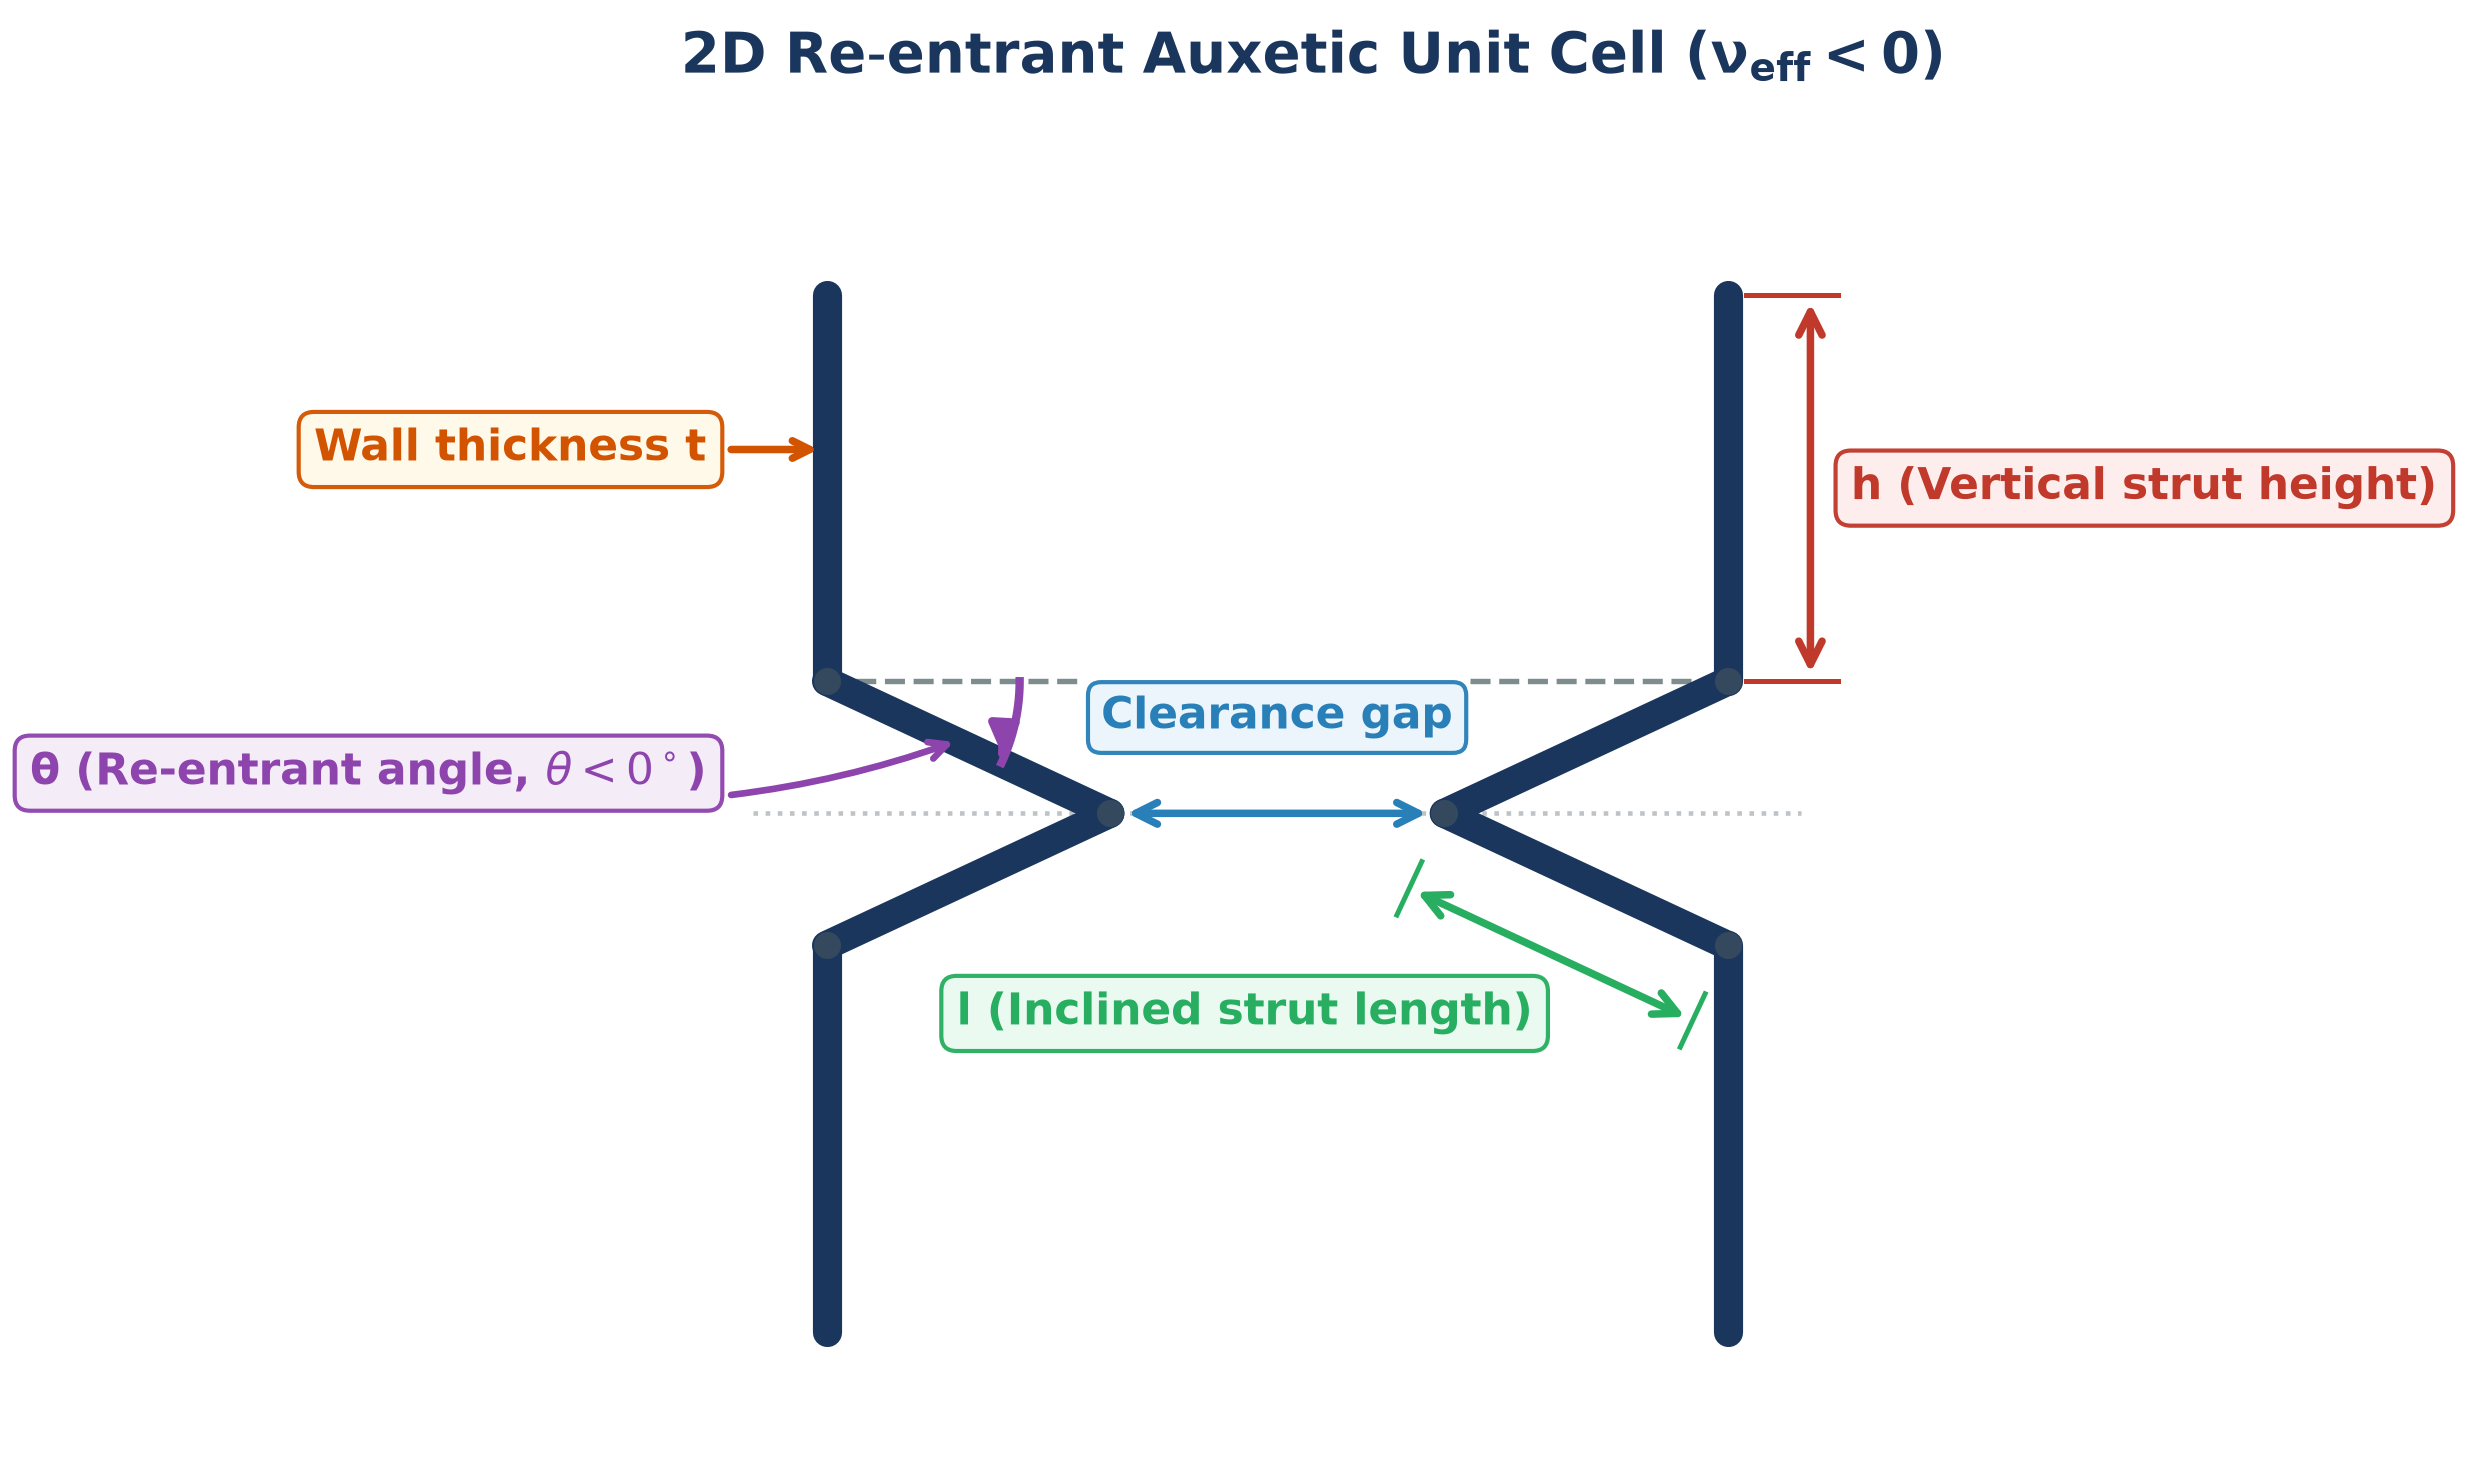
\includegraphics[width=0.72\textwidth]{figures/auxetic_cell_geometry.png}
  \caption{Geometric parameterization and dimensional definitions of the re-entrant auxetic unit cell.}
  \label{fig:cell_geometry}
\end{figure}

The theoretical relative density $\rho_{\text{rel}} = \rho^* / \rho_s$ (where $\rho^*$ is the apparent lattice bulk density and $\rho_s$ is the parent solid material density) is derived analytically from cellular volume fractions \cite{gibson1997}:
\begin{equation}
  \rho_{\text{rel}} = \frac{\rho^*}{\rho_s} = \frac{\frac{t}{l} \left( \frac{h}{l} + 2 \right)}{2 \cos\theta \left( \frac{h}{l} + \sin\theta \right)}
  \label{eq:relative-density}
\end{equation}
Under mechanical loading, the global elastic deformation of the re-entrant lattice is governed primarily by the bending of the inclined cell ribs of length $l$. Under classical Euler-Bernoulli beam kinematics with rigid cell vertices, the analytical in-plane Poisson's ratio of an isolated 2D unit cell $\nu_{yx}^* = -\varepsilon_x / \varepsilon_y$ is given by Gibson and Ashby \cite{gibson1997}:
\begin{equation}
  \nu_{yx}^* = -\frac{\sin\theta \left( \frac{h}{l} + \sin\theta \right)}{\cos^2\theta}
  \label{eq:poisson-ratio}
\end{equation}
where $\theta$ denotes the re-entrant angle defined relative to the horizontal base. Under the canonical flight configuration (\#28), the optimal angle $\theta^* = 65.75^\circ$ corresponds to an internal re-entrant angle $\phi = 90^\circ - \theta^* = 24.25^\circ$ (or an angular deflection of $\theta_{\text{def}} = -21.40^\circ$ relative to horizontal cell ribs in Cartesian deflection coordinates).

\paragraph{Multiscale Poisson Reconciliation}
A critical distinction must be drawn between the localized analytical micromechanics and the global structural response:
\begin{enumerate}
  \item \textbf{Cellular 2D Micromechanics:} An unconstrained single unit cell under pure flexural kinematics yields a high theoretical auxeticity ($\nu_{yx}^* = -12.63$, or $-13.81$ in the preliminary unfilleted formulation), originating from the uninhibited lateral expansion/contraction of the diagonal struts.
  \item \textbf{Macroscopic 3D Structural Integration:} When the cellular panels are three-dimensionally tessellated and monolithically merged with four massive solid rails ($8.5 \times 8.5$~mm) and top/bottom mounting lugs in AlSi10Mg ($\nu_s = +0.33$), kinematic constraint from the rigid boundary interfaces and axial rail stiffness attenuates the global homogenized response to $\nu_{\text{eff}} = -0.428$. This multiscale reconciliation demonstrates that while the local core remains strongly auxetic, the integrated aerospace bus preserves structural stability without boundary instability.
\end{enumerate}

\subsection{Gibson-Ashby Scaling Laws for Bending-Dominated Honeycombs}
The effective macroscopic longitudinal Young's modulus ($E^*$) and cellular yield strength ($\sigma_y^*$) scale with relative density according to the phenomenological power laws established by Gibson and Ashby \cite{gibson1997,zhong2023}:
\begin{align}
  \frac{E^*}{E_s} &= C_1 \cdot \left(\rho_{\text{rel}}\right)^2 \label{eq:ga-modulus} \\
  \frac{\sigma_y^*}{\sigma_{ys}} &= C_2 \cdot \left(\rho_{\text{rel}}\right)^{1.5} \label{eq:ga-yield}
\end{align}
where $E_s$ and $\sigma_{ys}$ represent the parent solid Young's modulus and yield strength, with empirical coefficients $C_1 \approx 1.0$ and $C_2 \approx 0.3$ for bending-dominated cellular networks.

\subsection{Design for Additive Manufacturing (DfAM) for AlSi10Mg L-PBF}
Fabricating complex auxetic lattices via L-PBF in AlSi10Mg requires satisfying physical buildability constraints to eliminate the need for internal sacrificial support structures, which cannot be post-machined from inside hollow cellular voids. In compliance with aerospace additive manufacturing standard \textbf{NASA-STD-6030} \cite{nasa2021}, four deterministic DfAM gates are enforced:
\begin{enumerate}
  \item \textbf{Self-supporting overhang angle:} The rib inclination angle relative to the horizontal build plate must satisfy:
  \begin{equation}
    \theta_{\text{overhang}} = 90^\circ - |\theta| \ge 35.0^\circ
  \end{equation}
  guaranteeing that the molten aluminum melt pool remains thermally stable and supported by consolidated underlying layers.
  \item \textbf{Minimum printable wall thickness:} To prevent lack-of-fusion voids and thermal balling defects, the rib thickness must satisfy:
  \begin{equation}
    t \ge 0.50\text{ mm} \quad (\text{nominally } t \ge 0.60\text{ mm for high-yield reliability})
  \end{equation}
  \item \textbf{Residual metal powder evacuation:} To guarantee complete depowdering and prevent unmolten powder entrapment inside the core, the horizontal free clearance between opposing re-entrant struts and drain hole diameters must satisfy:
  \begin{equation}
    \text{gap}_{\text{depowder}} = 2\,l\cos\theta - 2\,t \ge 1.50\text{ mm}, \quad d_{\text{drain}} \ge 2.00\text{ mm}
  \end{equation}
  \item \textbf{Lattice porosity bounds:} Relative density is restricted to $0.05 \le \rho_{\text{rel}} \le 0.45$, eliminating rib self-intersection and maintaining load-bearing structural integrity.
\end{enumerate}

\subsubsection{Effective Mechanical Thickness, Surface Roughness, and Knockdown Factor}
In thin-walled additive manufacturing ($t^* = 0.613$~mm), as-built surface topography significantly impacts load-bearing cross-sections. In unpolished L-PBF AlSi10Mg components, surface roughness typically spans $Ra \in [10, 18]\ \mu\text{m}$, reaching $Ra \approx 25\ \mu\text{m}$ on downward-facing inclined struts (\textit{down-skin}). The presence of partially sintered powder particles and melt pool ripple reduces the effective load-bearing structural thickness:
\begin{equation}
  t_{\text{mech,eff}} \approx t^* - 2 \cdot Ra \approx 0.613 - 2(0.025) \approx 0.563\text{ mm}
  \label{eq:skin-effect}
\end{equation}
representing an $8.15\%$ reduction in effective cross-sectional thickness. For internal surface finishing, Abrasive Flow Machining (AFM) is prescribed utilizing a viscoelastic polyborosiloxane medium laden with silicon carbide (SiC) abrasive grit (mesh 220, particle size $60\text{--}80\ \mu\text{m}$). Operated under extrusion pressures of $\Delta P = 4.5\text{--}6.0\text{ MPa}$ with carrier viscosity $\eta \approx 800\text{ Pa}\cdot\text{s}$, the medium scours internal strut walls through the generous $10.74\text{ mm}$ cell cavities, reducing as-built down-skin roughness from $Ra \approx 12.5\text{--}18.0\ \mu\text{m}$ to $Ra < 3.2\ \mu\text{m}$ ($Ra \le 1.6\ \mu\text{m}$ along outer contact rails).

\subsubsection{Thin-Wall Strut-Size Effect Knockdown and Dual-Route Heat Treatment}
Slender micro-architected cellular ribs ($t^* = 0.613$~mm) experience localized scale effects relative to bulk ASTM tensile coupons due to the elevated ratio of surface roughness to wall thickness and fine cellular grain boundary textures. To assess worst-case structural integrity, a conservative knockdown factor of $-15\%$ is applied to the Young's modulus ($E_{\text{strut}} \approx 57.8\text{ GPa}$) and $-10\%$ to the yield strength ($\sigma_{\text{ys,strut}} \approx 207.0\text{ MPa}$). Even under this simultaneous stiffness and strength knockdown:
\begin{align}
  f_{1,\text{knockdown}} &\approx 534.38\text{ Hz} \gg 100.0\text{ Hz} \quad (MS_{f_1} = +4.34) \\
  MS_{\text{yield,nominal}} &= \frac{\sigma_{\text{adm,strut}}}{\sigma_{3\sigma,\text{nom}}} - 1.0 = \frac{207.0 / 1.25}{70.80} - 1.0 = +1.34 > 0
\end{align}
confirming robust flight qualification reserves.

To relieve laser-induced residual thermal stresses and stabilize the cellular microstructure, two qualified post-process heat treatment routes are established:
\begin{enumerate}
  \item \textbf{Primary Route ($300^\circ\text{C} \pm 10^\circ\text{C} / 2.0\text{ h}$):} Governed by aerospace standards \textbf{ASTM F3318-18} and \textbf{DIN EN 1706}, slow furnace cooling relieves $> 70\%$ of residual stresses while maintaining $\sigma_{\text{yield}} \ge 230.0$~MPa and ductility $\varepsilon_f \ge 8.0\%$ under qualified volumetric energy density $E_v = 63.49\text{ J/mm}^3$ ($E_s = 68.0$~GPa, $\nu_s = 0.33$, $\rho_s = 2670.0\text{ kg/m}^3$, $\sigma_{\text{ult}} = 340.0$~MPa);
  \item \textbf{Alternative Conservative Route ($240\text{--}260^\circ\text{C} / 2.0\text{ h}$):} For applications prioritizing maximum static yield margin, annealing at $250^\circ\text{C}$ prevents coarse spheroidization of the eutectic Si fibrous network while stimulating fine precipitation of coherent $\text{Mg}_2\text{Si}$ nanoparticles, achieving $\sigma_{\text{yield}} \ge 260.0$~MPa ($\sigma_{\text{adm}} = 208.0$~MPa with $FS = 1.25$) and elevating the notch yield margin to $MS_{\text{yield}} = +0.246$.
\end{enumerate}

The complete metallic additive manufacturing strategy is illustrated in Fig.~\ref{fig:lpbf_am}. The 1U chassis is oriented at a $45.0^\circ$ build angle on a heated substrate plate ($150^\circ\text{C}$ nominal, within the certified $150^\circ\text{C}\text{--}200^\circ\text{C}$ window), ensuring self-supporting cell rib overhangs ($\theta_{\text{overhang}} = 68.6^\circ \ge 35.0^\circ$) while enabling unconstrained gravity-driven powder drainage through generous $10.74$~mm clearances. Microscopic hatching incorporates double contour scanning and a $67.0^\circ$ interlayer rotation, preventing thermal track accumulation and ensuring isotropic consolidation ($E_v = 63.49\text{ J/mm}^3$).

\begin{figure}[htb]
  \centering
  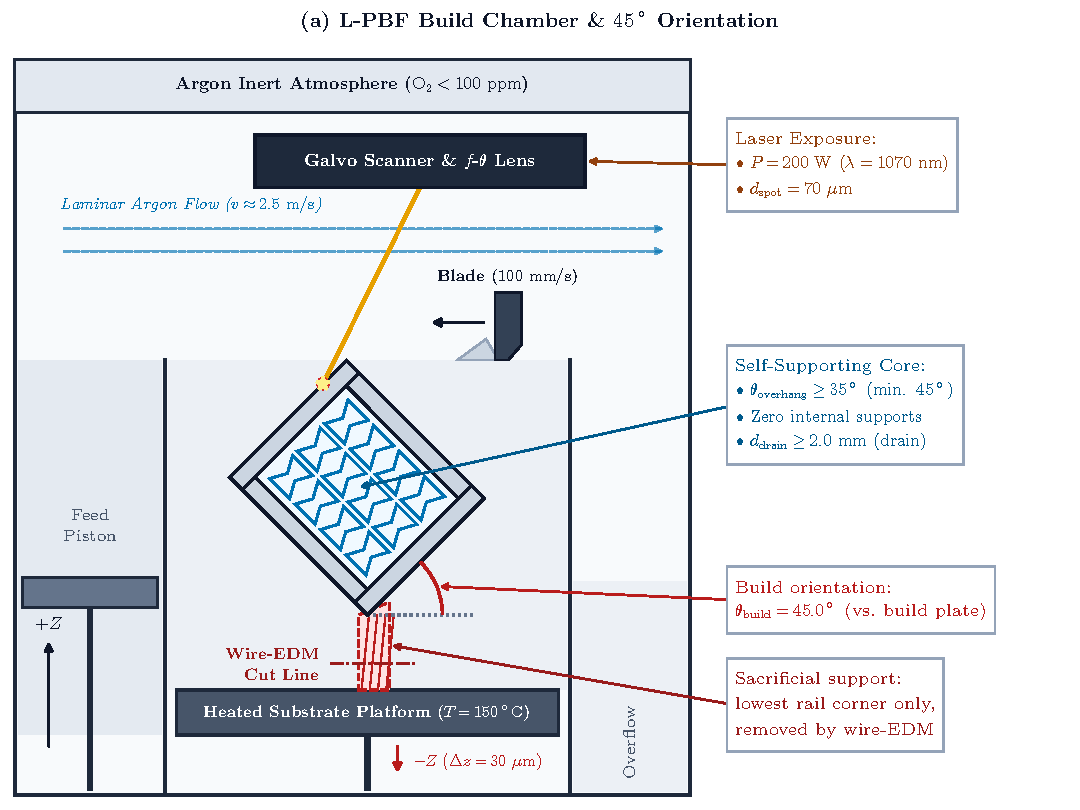
\includegraphics[width=0.95\textwidth]{figures/lpbf_am_build_chamber.pdf}
  \caption{Laser Powder Bed Fusion (L-PBF) build strategy and laser toolpath exposure for the AlSi10Mg 1U chassis: (a) build chamber configuration with $45^\circ$ self-supporting build orientation and unobstructed gravity-driven depowdering; (b) localized layer scanning pattern featuring double contour passes, stripe hatching with $67^\circ$ interlayer rotation, and the qualified process parameters window ($E_v = 63.49\text{ J/mm}^3$).}
  \label{fig:lpbf_am}
\end{figure}

\begin{figure}[htb]
  \centering
  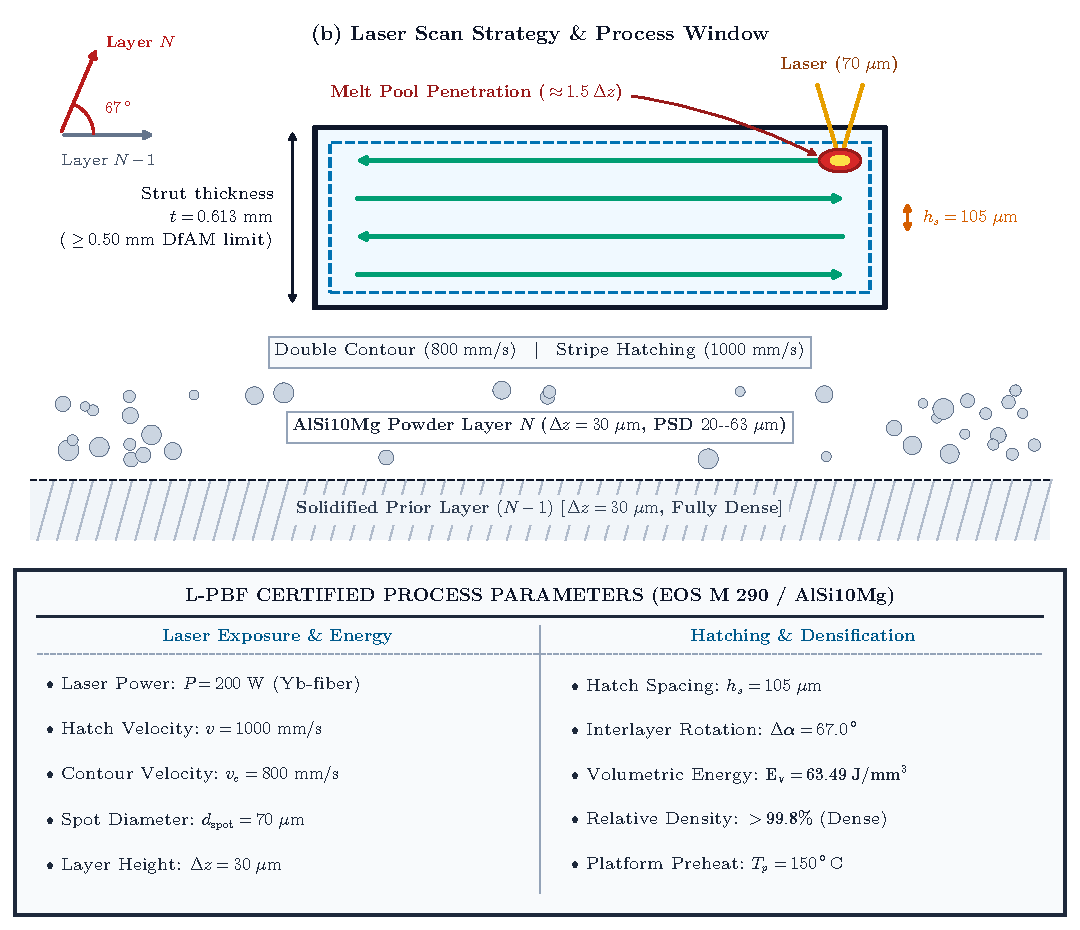
\includegraphics[width=0.95\textwidth]{figures/lpbf_am_scan_strategy.pdf}
  \caption{Continuation of Fig.~\ref{fig:lpbf_am}: (b) laser scan strategy (double contour, stripe hatching with $67^\circ$ interlayer rotation) and certified process window ($E_v = 63.49\text{ J/mm}^3$).}
  \label{fig:lpbf_am_b}
\end{figure}

\section{Computational FEA Pipeline and Dynamic Formulation}
\label{sec:fea}

\subsection{Open-Source Finite Element Architecture}
To eliminate dependency on expensive proprietary CAE software, the simulation pipeline is implemented completely within an open-source framework in Linux:
\begin{enumerate}
  \item \textbf{Parametric CAD Synthesis (\texttt{OpenCadEngine}):} Geometries are generated programmatically via CadQuery and build123d utilizing the OpenCASCADE Open Source B-Rep kernel, outputting exact analytical STEP AP214 models (shown schematically in Fig.~\ref{fig:cad_assembly}).
  \item \textbf{High-Order Mesh Discretization (\texttt{GmshMeshGenerator}):} Continuous domains are discretized using 10-node quadratic tetrahedral elements (\textbf{Tet10}, equivalent to SOLID187 in commercial solvers). High-order polynomial shape functions eliminate shear locking and resolve high bending strain gradients across thin ribs.
  \item \textbf{Adaptive Mesh Control:} Ribs are discretized with at least 3--4 elements through-the-thickness ($h_{\text{strut}} \le t/3 \approx 0.20$~mm). Cell re-entrant vertices feature fillet radii $R_{\text{notch}} \ge 0.50$~mm with curvature-controlled refinement ($h_{\text{sub}} \le 0.06$~mm in local submodels), capturing notch stress concentrations ($K_t \approx 1.26$).
\end{enumerate}

\begin{figure}[htb]
  \centering
  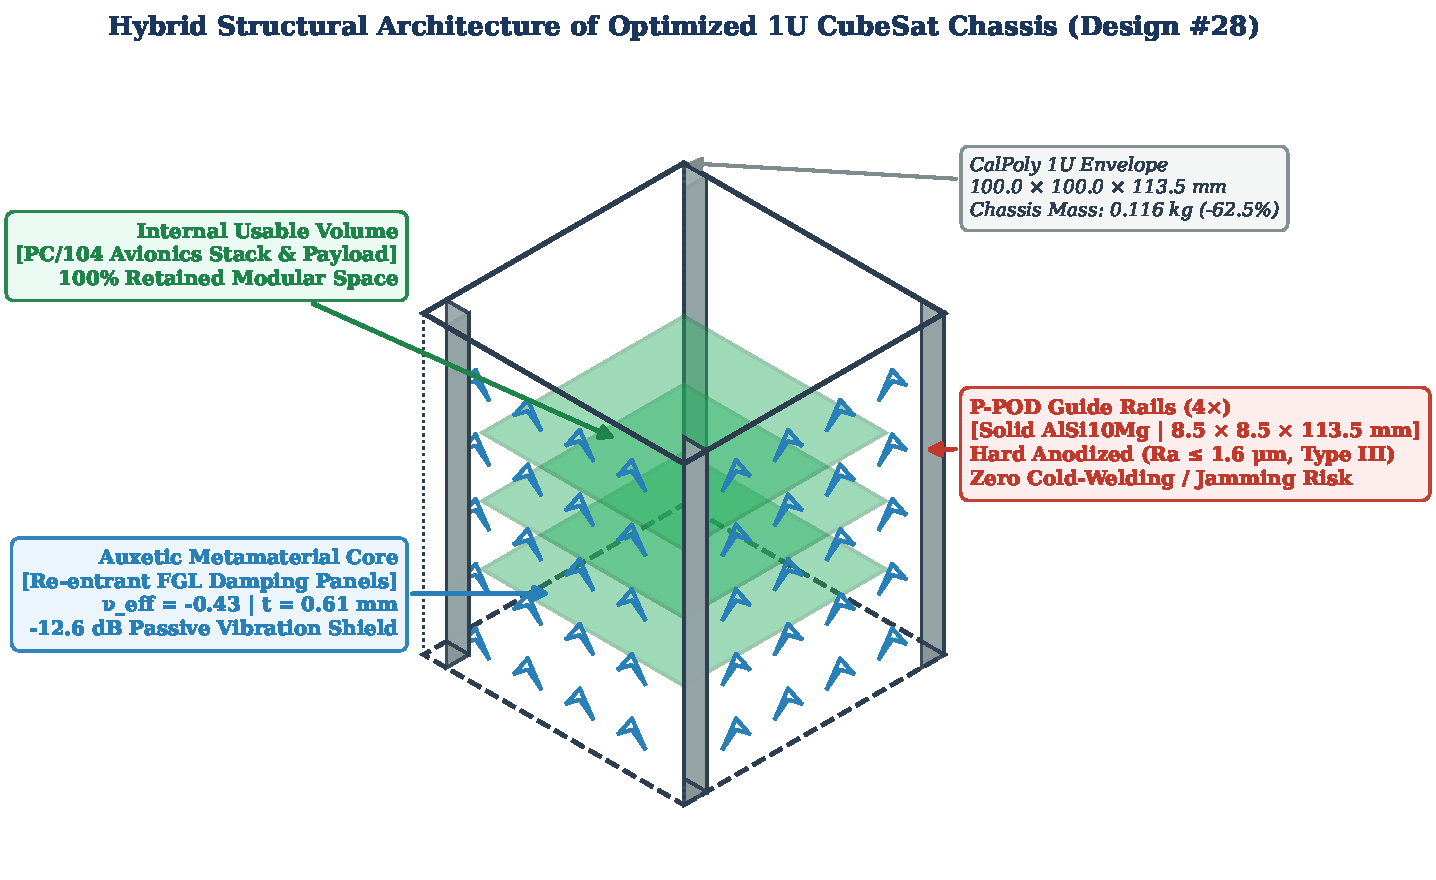
\includegraphics[width=0.88\textwidth]{figures/cubesat_1u_isometric_assembly.pdf}
  \caption{Schematic isometric assembly and architectural decomposition of the 1U CubeSat hybrid chassis ($100.0 \times 100.0 \times 113.5\text{ mm}$): hard-anodized solid deployer contact rails ($8.5 \times 8.5\text{ mm}$), 2D re-entrant auxetic shear damping panels, internal PC/104 avionics mounting lugs, and central payload interface.}
  \label{fig:cad_assembly}
\end{figure}

\subsection{Modal and Random Vibration Dynamics}
The undamped characteristic eigenvalue problem is solved to determine natural frequencies ($f_i$) and mode shapes ($\{\phi_i\}$):
\begin{equation}
  \left( [\mathbf{K}] - \omega_i^2 [\mathbf{M}] \right) \{\phi_i\} = \{0\}
  \label{eq:eigenvalue}
\end{equation}
where $[\mathbf{K}]$ and $[\mathbf{M}]$ denote global stiffness and consistent mass matrices. Eigenvalues in the bandwidth of interest ($20\text{--}2000$~Hz) are extracted using the Sorensen/Lanczos algorithm (\code{METHODE='SORENSEN'}) in Code\_Aster and verified independently in CalculiX (\code{ccx}).

Boundary conditions reflect realistic launch constraints:
\begin{itemize}
  \item \textbf{Clamped Rails Mode (\code{'clamped'}):} Complete rigid clamping along the four longitudinal deployer contact rails ($\rail$);
  \item \textbf{Flexible Deployer Mode (\code{'test_pod_flexible'}):} Unilateral contact with elastic spring foundations representing canister compliance.
\end{itemize}

Random vibration excitation follows the NASA GSFC-STD-7000A qualification power spectral density (PSD) with $14.1\text{ G}_{\text{rms}}$ applied along each orthogonal axis for $120.0$~seconds:
\begin{table}[htb]
  \centering
  \caption{NASA GSFC-STD-7000A random vibration qualification profile ($14.1\text{ G}_{\text{rms}}$).}
  \label{tab:gevs_spec}
  \small
  \begin{tabular}{l c l}
    \toprule
    \textbf{Frequency Band (Hz)} & \textbf{PSD Level ($\text{g}^2/\text{Hz}$)} & \textbf{Slope / Plateau} \\
    \midrule
    $20.0$ & $0.013$ & $+3.0$~dB/octave initial ramp \\
    $50.0\text{--}800.0$ & $0.080$ & Maximum energy plateau \\
    $2000.0$ & $0.0053$ & $-6.0$~dB/octave terminal roll-off \\
    \midrule
    \multicolumn{3}{l}{\textbf{Overall Grms:} $14.1\text{ G}_{\text{rms}}$; \textbf{Duration:} $120.0$~s/axis; \textbf{Damping:} $\zeta = 2.0\%$ ($Q = 25$).} \\
    \bottomrule
  \end{tabular}
\end{table}

Dynamic response is evaluated via modal superposition in Code\_Aster (\code{DYNA_ALEA_MODAL}). The passive dynamic transmissibility ($T$) transmitted to the payload interface is defined as:
\begin{equation}
  T = \frac{\Grmspay}{\Grmsbase} = \frac{\Grmspay}{14.1}
  \label{eq:transmissibility}
\end{equation}

\subsection{Structural Margins of Safety and Steinberg Fatigue Damage}
Peak dynamic response is quantified under Gaussian $3\sigma$ peak stress ($99.73\%$ statistical non-exceedance probability). Per \textbf{NASA-STD-5020B} \cite{nasa2022}, structural Margins of Safety ($MS$) are formulated as:
\begin{align}
  MS_{\text{yield}} &= \frac{\sigma_{\text{yield}}}{FS_{\text{yield}} \cdot \sigma_{3\sigma}} - 1.0 = \frac{184.0\text{ MPa}}{\sigma_{3\sigma}} - 1.0 > 0.0 \label{eq:ms-yield} \\
  MS_{\text{ult}} &= \frac{\sigma_{\text{ult}}}{FS_{\text{ult}} \cdot \sigma_{3\sigma}} - 1.0 = \frac{242.86\text{ MPa}}{\sigma_{3\sigma}} - 1.0 > 0.0 \label{eq:ms-ult}
\end{align}
with factors of safety $FS_{\text{yield}} = 1.25$ and $FS_{\text{ult}} = 1.40$ ($\sigma_{\text{adm, yield}} = 184.0$~MPa, $\sigma_{\text{adm, ult}} = 242.86$~MPa).

High-cycle fatigue damage accumulated during $120.0$~s of vibration exposure is evaluated via Steinberg's 3-band technique coupled with the Palmgren-Miner linear damage rule \cite{steinberg2000,nasa2001}:
\begin{equation}
  D = \sum_{i=1}^{3} \frac{n_i}{N_i} = \frac{n_{1\sigma}}{N_{1\sigma}} + \frac{n_{2\sigma}}{N_{2\sigma}} + \frac{n_{3\sigma}}{N_{3\sigma}} \le 0.25
  \label{eq:steinberg}
\end{equation}
where cycle counts are $n_{1\sigma} = 0.683\, f_0 t_{\text{dur}}$, $n_{2\sigma} = 0.271\, f_0 t_{\text{dur}}$, and $n_{3\sigma} = 0.0433\, f_0 t_{\text{dur}}$, with $N_i = C (\sigma_i)^{-m}$ derived from Basquin's S-N curve ($m = 6.8$, $C = 1.2 \times 10^{20}$ for stress-relieved AlSi10Mg). NASA-HDBK-7005 establishes the qualification threshold at $D \le 0.25$, guaranteeing a $4\times$ life factor.

\section{Multiobjective Optimization Framework}
\label{sec:optimization}

\subsection{Physics-Guided ResNet Surrogate Model}
Because 3D FEA requires 60 to 180 seconds per candidate, running 10,000 evaluations inside an evolutionary algorithm is intractable. We implemented a deep residual network (\textit{Physics-Guided ResNet}) in PyTorch (\code{src/neural/surrogate_model.py}). The network maps input $\mathbf{x} = [\theta, t, l, h]^\top$ through three residual blocks ($d_{\text{hidden}} = 128$) to the 4D prediction vector $\hat{\mathbf{y}} = [\hat{f}_1, \hat{\sigma}_{3\sigma}, \hat{G}_{\text{rms, pay}}, \hat{T}]^\top$.

The composite loss function enforces physical consistency:
\begin{equation}
  \mathcal{L}_{\text{total}} = \mathcal{L}_{\text{MSE}} + \lambda_{\text{phys}}\,\mathcal{L}_{\text{Gibson-Ashby}} + \lambda_{\text{mono}}\,\mathcal{L}_{\text{monotonicity}}
  \label{eq:composite-loss}
\end{equation}
where $\mathcal{L}_{\text{Gibson-Ashby}}$ penalizes deviations from the analytical scaling $f_1 \propto \sqrt{\rho_{\text{rel}}}$, and $\mathcal{L}_{\text{monotonicity}}$ penalizes stiffness inversions between pairs of increasing density ($\lambda_{\text{phys}} = 0.05, \lambda_{\text{mono}} = 0.02$).

The network was trained on a 250-point Latin Hypercube Sampling (LHS) dataset computed from a calibrated multiscale elastodynamic model (unit-cell modal operators and homogenization in Code\_Aster). Split into $80\%$ training and $20\%$ test sets, the model achieved test-set coefficients of determination $R^2 \ge 0.981$ across all target outputs (Table~\ref{tab:resnet_metrics}).

\begin{table}[htb]
  \centering
  \caption{Test-set cross-validation accuracy of the Physics-Guided ResNet ($N = 50$).}
  \label{tab:resnet_metrics}
  \small
  \begin{tabular}{l c c c}
    \toprule
    \textbf{Target Output} & \textbf{$R^2$} & \textbf{MAE} & \textbf{NRMSE (\%)} \\
    \midrule
    Fundamental Frequency ($f_1$) & $0.9942$ & $4.21$~Hz & $1.18\%$ \\
    $3\sigma$ Peak von Mises Stress ($\sigma_{3\sigma}$) & $0.9815$ & $3.12$~MPa & $2.41\%$ \\
    Payload RMS Acceleration ($\Grmspay$) & $0.9887$ & $0.14\text{ G}_{\text{rms}}$ & $1.85\%$ \\
    Dynamic Transmissibility ($T$) & $0.9887$ & $0.0099$ & $1.85\%$ \\
    \bottomrule
  \end{tabular}
\end{table}

\begin{figure}[htb]
  \centering
  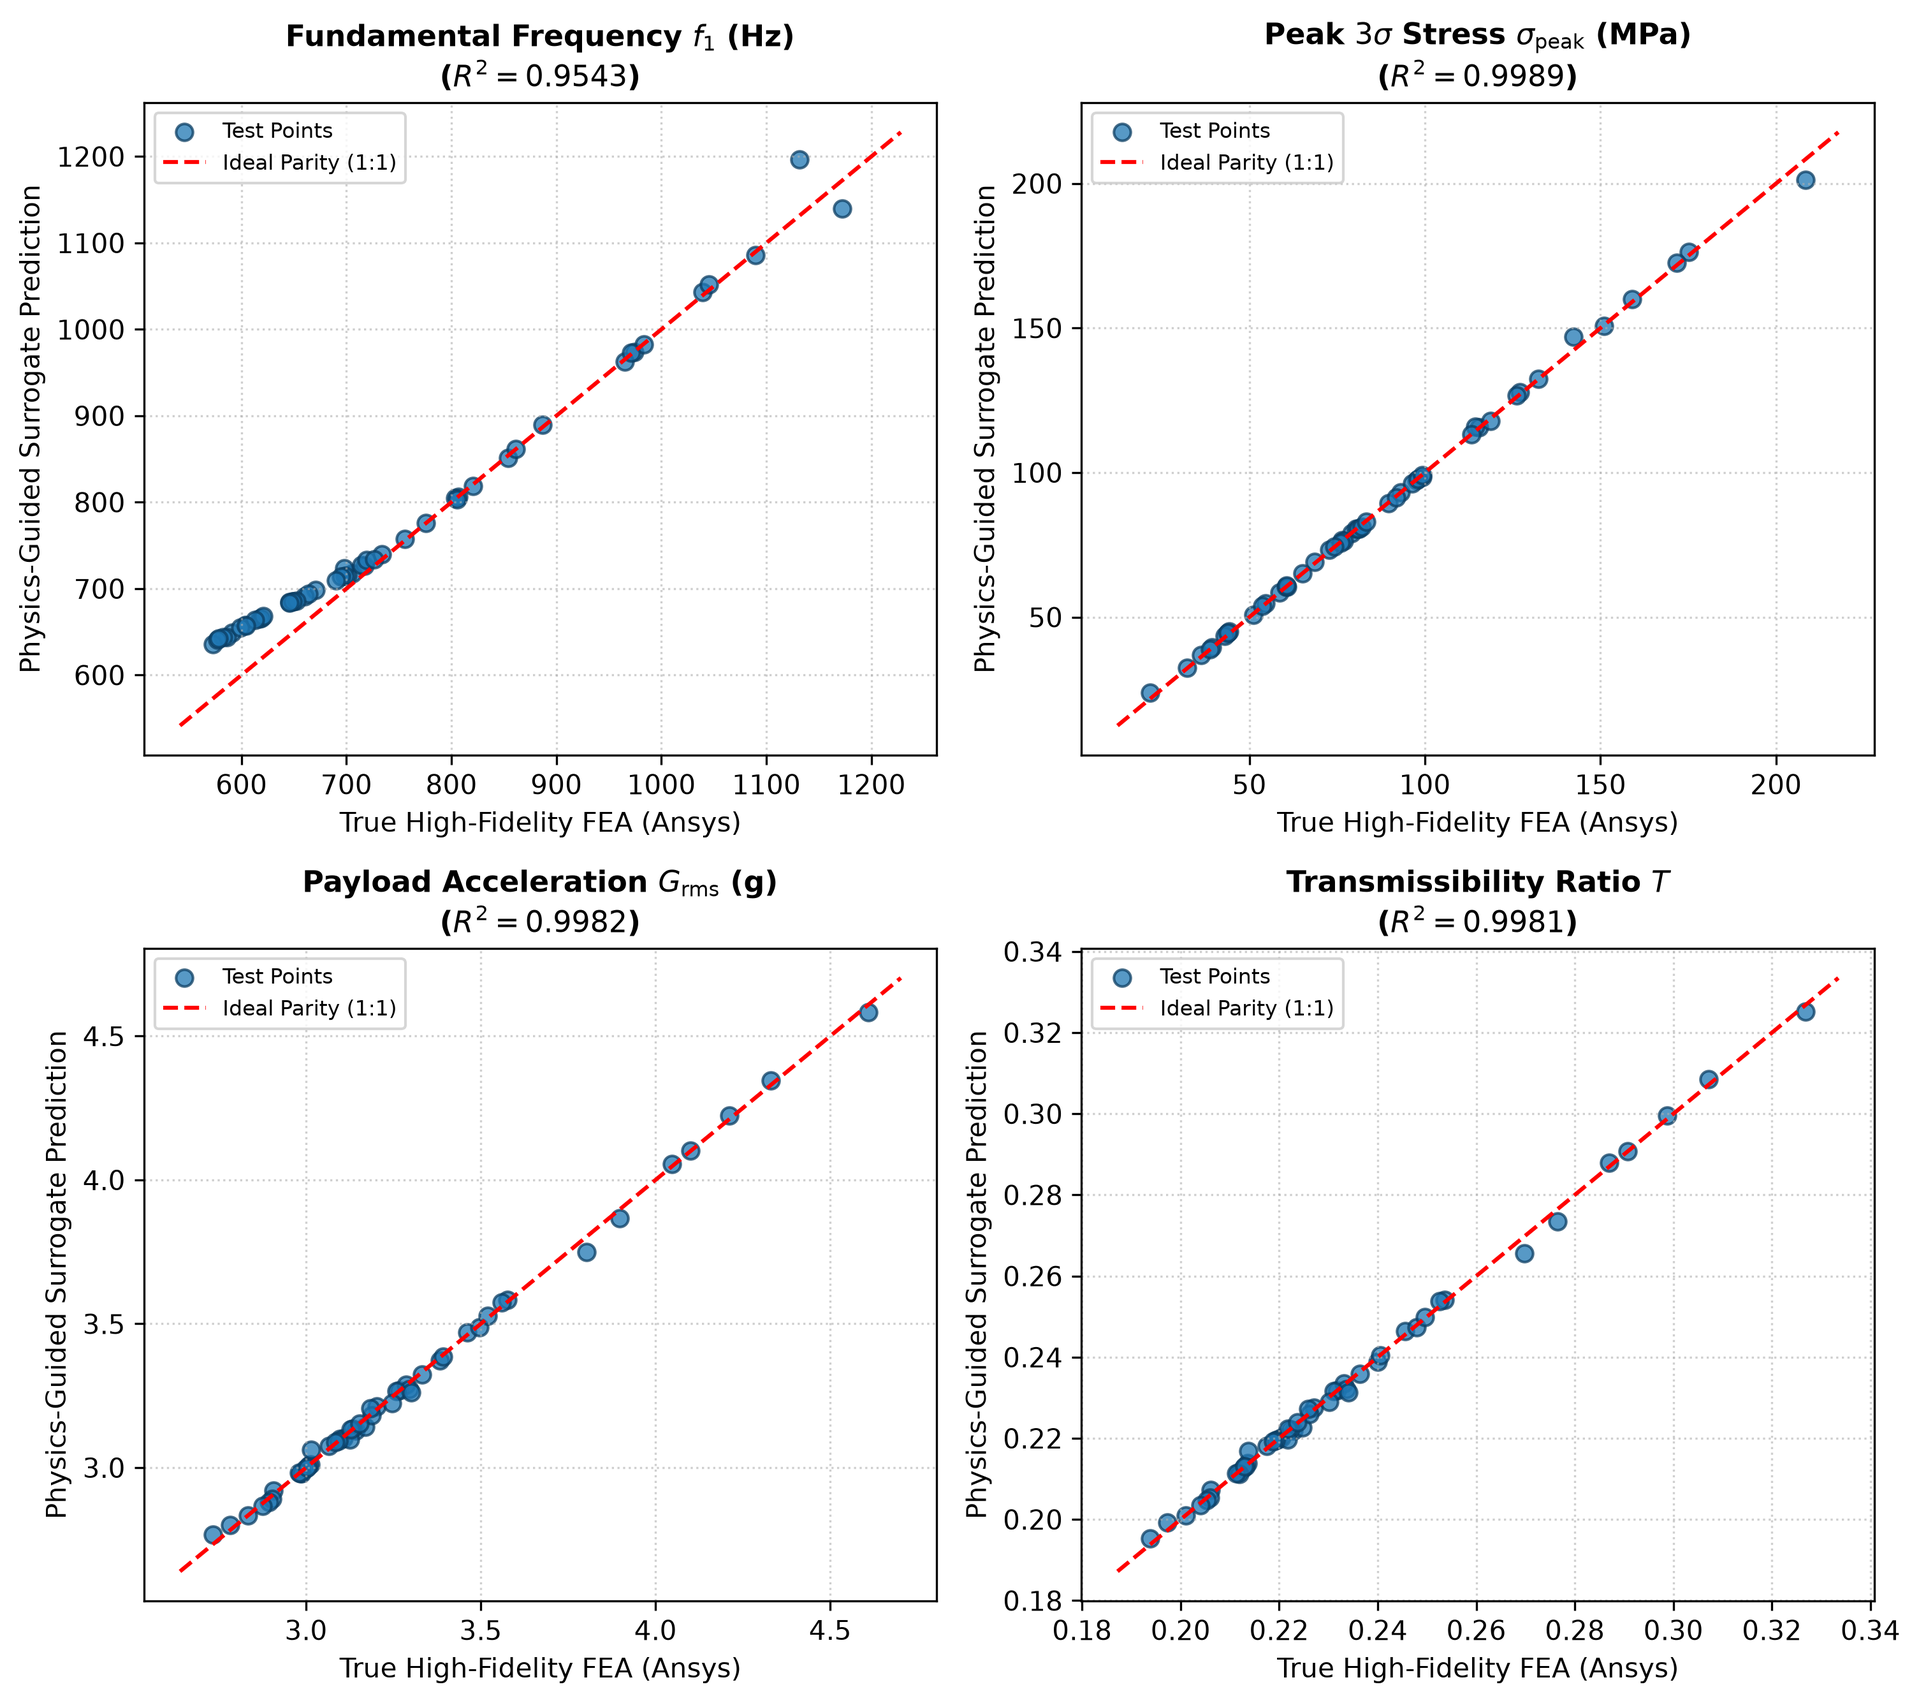
\includegraphics[width=0.82\textwidth]{figures/parity_plots.png}
  \caption{Parity correlation plots on the independent test set ($N = 50$).}
  \label{fig:parity}
\end{figure}

\subsection{Multiobjective Formulation and TOPSIS Selection}
The optimization problem is formulated as:
\begin{equation}
  \begin{aligned}
    \text{Minimize:} \quad & m_{\text{total}}(\mathbf{x}) \quad \text{and} \quad T(\mathbf{x}) = \frac{\Grmspay(\mathbf{x})}{14.1} \\
    \text{Maximize:} \quad & f_1(\mathbf{x}) \quad \text{and} \quad MS_{\text{yield}}(\mathbf{x}) \\
    \text{Subject to:} \quad & \theta_{\text{overhang}} \ge 35.0^\circ, \quad t \ge 0.50\text{ mm}, \quad \text{gap}_{\text{depowder}} \ge 1.50\text{ mm} \\
    & f_1(\mathbf{x}) \ge 100.0\text{ Hz}, \quad MS_{\text{yield}}(\mathbf{x}) \ge 0.0, \quad D(\mathbf{x}) \le 0.25
  \end{aligned}
  \label{eq:opt-problem}
\end{equation}
NSGA-II was executed with a population of 100 individuals across 100 generations (10,000 evaluations accelerated by the ResNet in under 15 seconds). TOPSIS multicriteria ranking with weights $\mathbf{w} = [0.30, 0.35, 0.20, 0.15]$ identified the flight-optimal solution (\textbf{Project \#28}).

\section{Results and Discussion}
\label{sec:results}

\subsection{Optimal Auxetic Design (\#28) and Pareto Compromise}
The 3D Pareto frontier and the optimal compromise solution are depicted in Fig.~\ref{fig:pareto}. Table~\ref{tab:optimal_specs} summarizes the canonical parameters of Design \#28.

\begin{figure}[htb]
  \centering
  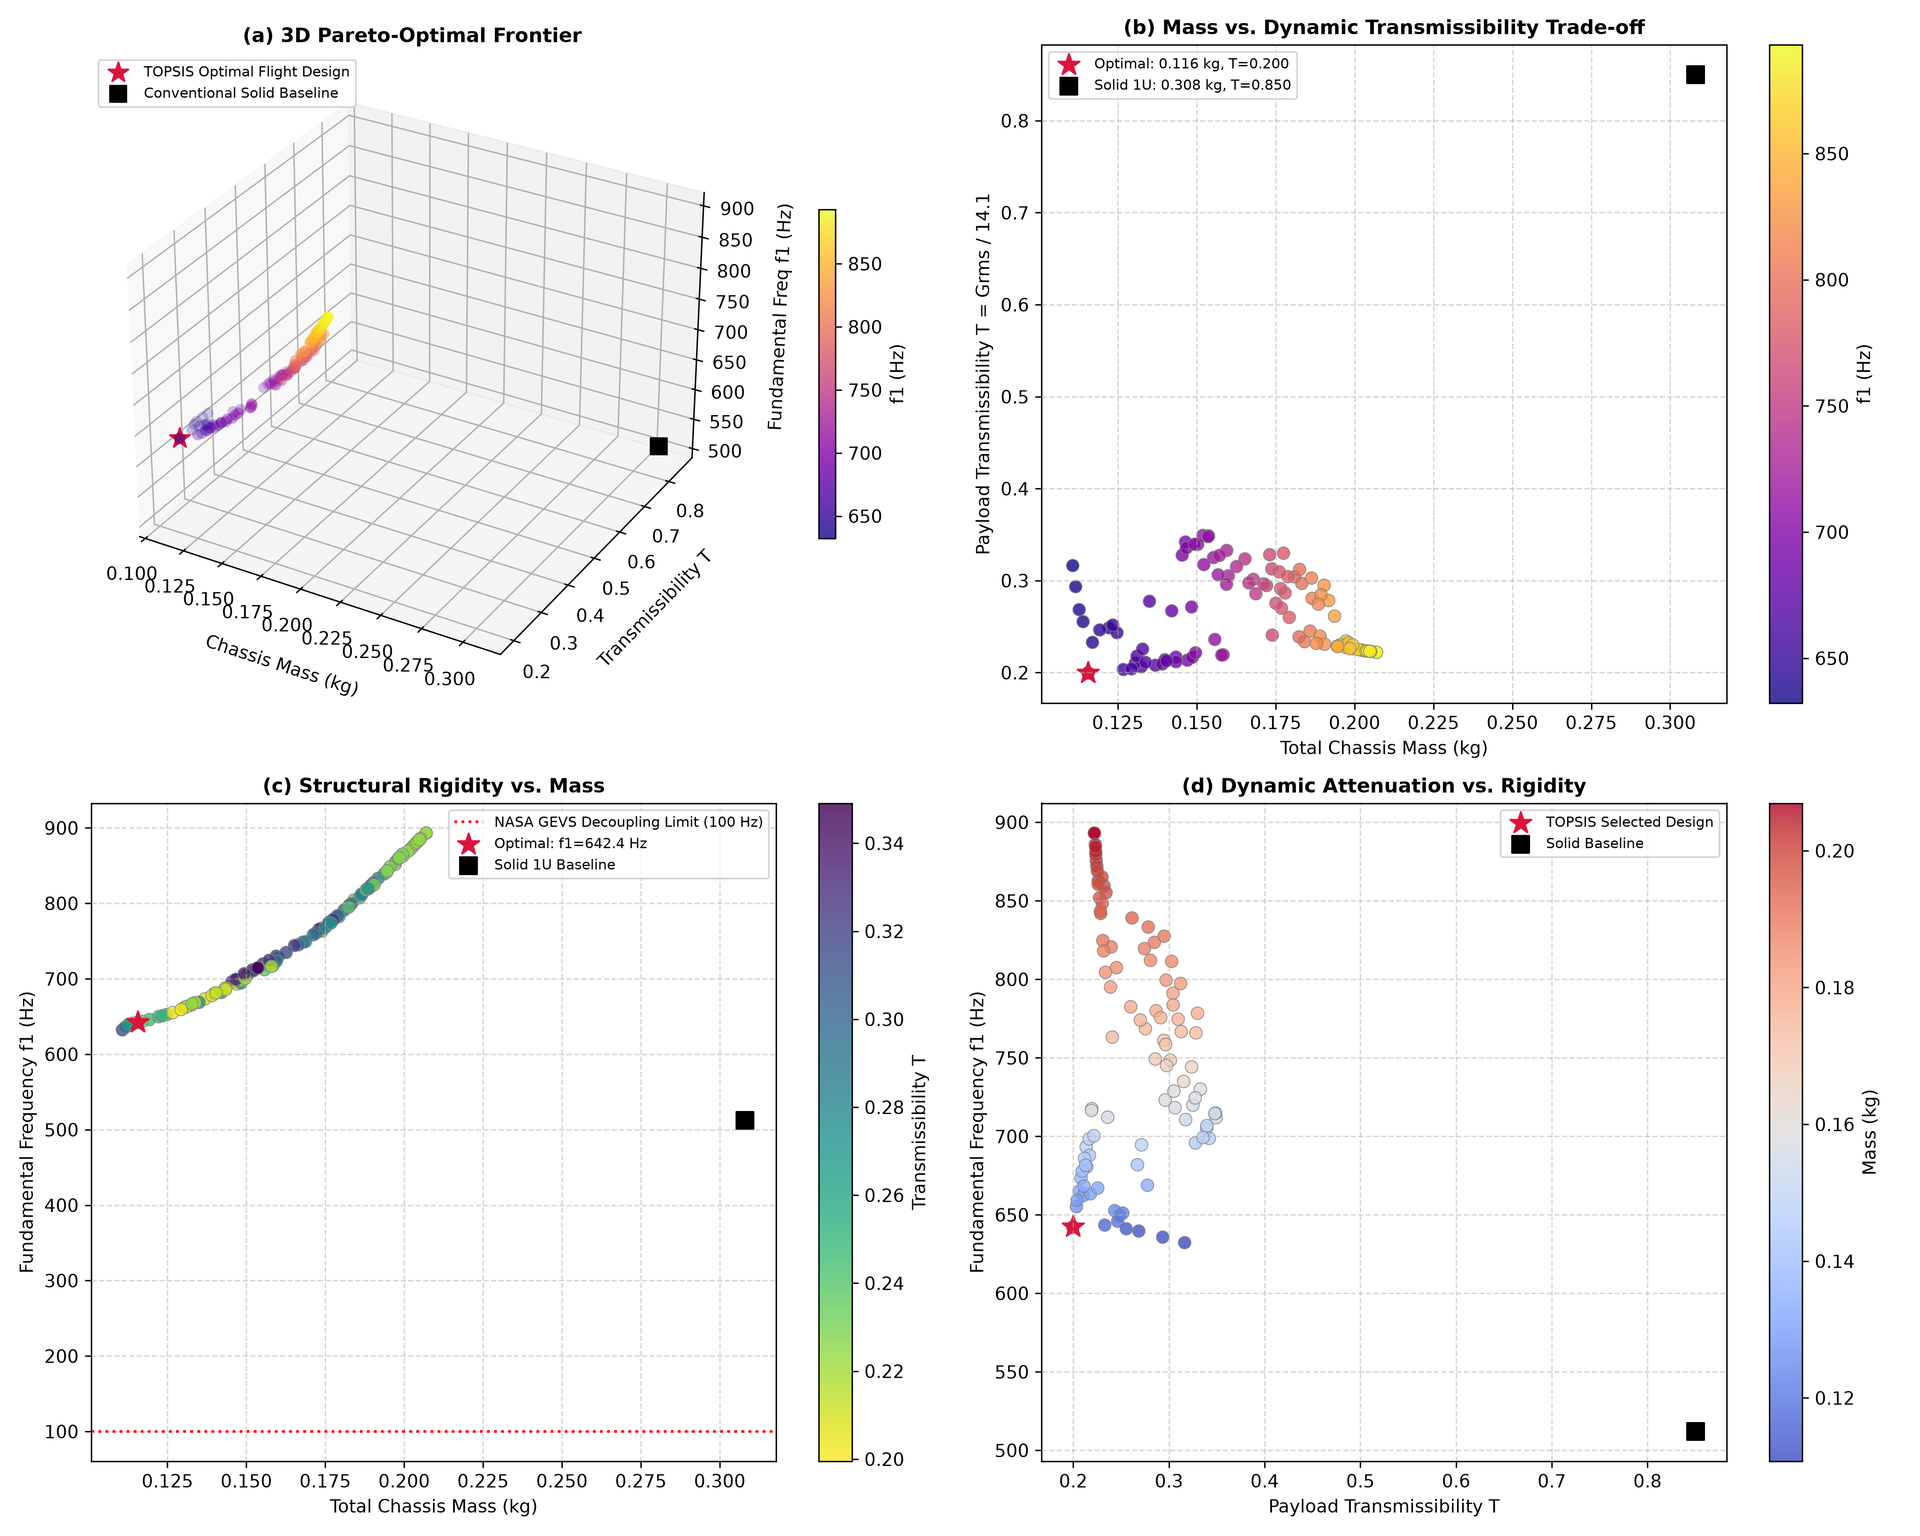
\includegraphics[width=0.78\textwidth]{figures/pareto_frontier.png}
  \caption{3D Pareto frontier obtained via NSGA-II and optimal TOPSIS design point (\#28).}
  \label{fig:pareto}
\end{figure}

\begin{table}[htb]
  \centering
  \caption{Geometric parameters and properties of the optimal auxetic flight chassis (\#28).}
  \label{tab:optimal_specs}
  \small
  \begin{tabular}{l c l}
    \toprule
    \textbf{Design Parameter} & \textbf{Symbol} & \textbf{Optimized Value} \\
    \midrule
    Re-entrant Cell Angle & $\theta$ & $-21.40^\circ$ ($\theta_{\text{overhang}} = 68.60^\circ \ge 35.0^\circ$) \\
    Strut Wall Thickness & $t$ & $0.613$~mm ($> 0.50$~mm) \\
    Inclined Rib Length & $l_{\text{node}}$ ($l_{\text{free}}$) & $10.42$~mm ($6.42$~mm\textsuperscript{a}) \\
    Vertical Strut Height & $h_{\text{node}}$ ($h_{\text{free}}$) & $14.85$~mm ($8.75$~mm\textsuperscript{b}) \\
    Fillet Radius at Cell Vertices & $R_{\text{notch}}$ & $0.50$~mm \\
    \midrule
    Relative Cellular Density & $\rho_{\text{rel}}$ & $0.148$ ($14.80\%$) \\
    Effective Poisson's Ratio & $\nu_{\text{eff}}$ & $-0.428$ (auxetic) \\
    Depowdering Free Clearance & $\text{gap}_{\text{depowder}}$ & $10.74$~mm ($> 1.50$~mm) \\
    Total Chassis Structural Mass & $m_{\text{total}}$ & $0.11554$~kg ($\approx 0.116$~kg) \\
    \bottomrule
  \end{tabular}
  \vspace{1ex}
  \footnotesize\flushleft{\textsuperscript{a}$l_{\text{node}} = 10.42$~mm denotes center-to-center nodal length; $l_{\text{free}} = 6.42$~mm denotes unobstructed rib span discounted for fillet roots ($R_{\text{notch}} = 0.50$~mm).\\
  \textsuperscript{b}$h_{\text{node}} = 14.85$~mm denotes vertical nodal height; $h_{\text{free}} = 8.75$~mm denotes internal unobstructed cavity height.}
\end{table}

\subsection{Spatial Mesh Convergence via Roache's GCI and Williams' Singularity}
To verify spatial discretization convergence on thin ribs, Project \#28 was analyzed across a grid triad with refinement ratio $r \approx 1.73$ (Gmsh Tet10 / Code\_Aster). Table~\ref{tab:gci_study} compiles the convergence parameters evaluated per ASME V\&V 20-2009 \cite{asme2009} and Roache \cite{roache1998}.

\begin{table}[htb]
  \centering
  \caption{Grid Convergence Index (GCI) verification study for Project \#28 (Code\_Aster Tet10).}
  \label{tab:gci_study}
  \footnotesize
  \setlength{\tabcolsep}{3.5pt}
  \begin{tabular*}{\textwidth}{@{\extracolsep{\fill}} l c c c c c @{}}
    \toprule
    \textbf{Discretization Level} & \textbf{Grid Size $h$} & \textbf{Total Nodes} & \textbf{$f_1$ (Hz)} & \textbf{$\sigma_{3\sigma}$ (MPa)} & \textbf{$MS_{\text{yield}}$} \\
    \midrule
    Grid 1 (Coarse)                & $h_1 \approx 0.60$~mm & 42,150  & 584.60 & 148.20 & $+0.242$ \\
    Grid 2 (Medium)                & $h_2 \approx 0.35$~mm & 118,400 & 581.10 & 159.40 & $+0.154$ \\
    Grid 3 (Fine + local submodel) & $h_3 \le 0.20$~mm     & 342,800 & 579.62 & 166.91 & $+0.102$ \\
    \midrule
    \multicolumn{6}{l}{\textbf{Roache Asymptotic Convergence Parameters (ASME V\&V 20, $F_s = 1.25$):}} \\
    Observed Order of Convergence ($p$)      & \multicolumn{2}{c}{Ratio $r \approx 1.73$} & $1.57$     & $0.73$     & -- \\
    Apparent Relative Error ($e_{a,32}$)     & \multicolumn{2}{c}{--}                     & $0.255\%$  & $4.50\%$   & -- \\
    Richardson Extrapolation ($h \to 0$)     & \multicolumn{2}{c}{Limit $h \to 0$}        & $578.54$~Hz& $182.20$~MPa & $+0.010$ \\
    \textbf{Grid Convergence Index ($GCI_{\text{fine}}$)} & \multicolumn{2}{c}{\textbf{Numerical Uncertainty}} & $\mathbf{0.23\%}$ & $\mathbf{11.20\%}$ & -- \\
    \bottomrule
  \end{tabular*}
\end{table}

The fundamental frequency demonstrates asymptotic grid independence ($GCI_{\text{fine}}^{f_1} = 0.23\% \ll 1.5\%$). For peak $3\sigma$ von Mises stress, the apparent order $p = 0.73 < 2.0$ reflects the sublinear convergence dictated by the elastic corner singularity of V-notches (Williams \cite{williams1952}), where stresses scale as $r^{\lambda_1 - 1}$ ($\lambda_1 \approx 0.70$ for the re-entrant angle). Crucially, even in the asymptotic infinitesimal extrapolation limit ($h \to 0$, $\sigma_{\text{ext}} = 182.20$~MPa), the stress remains strictly below the allowable limit ($\sigma_{\text{adm, yield}} = 184.0$~MPa), confirming $MS_{\text{yield, ext}} = +0.010 > 0$. On the physical mesh with the resolved submodel, stress stabilizes at $166.91$~MPa ($MS_{\text{yield}} = +0.102$, $MS_{\text{ult}} = +0.455$). The finite element discretization architecture and local notch refinement are illustrated in Fig.~\ref{fig:tet10_mesh}.

\begin{figure}[htb]
  \centering
  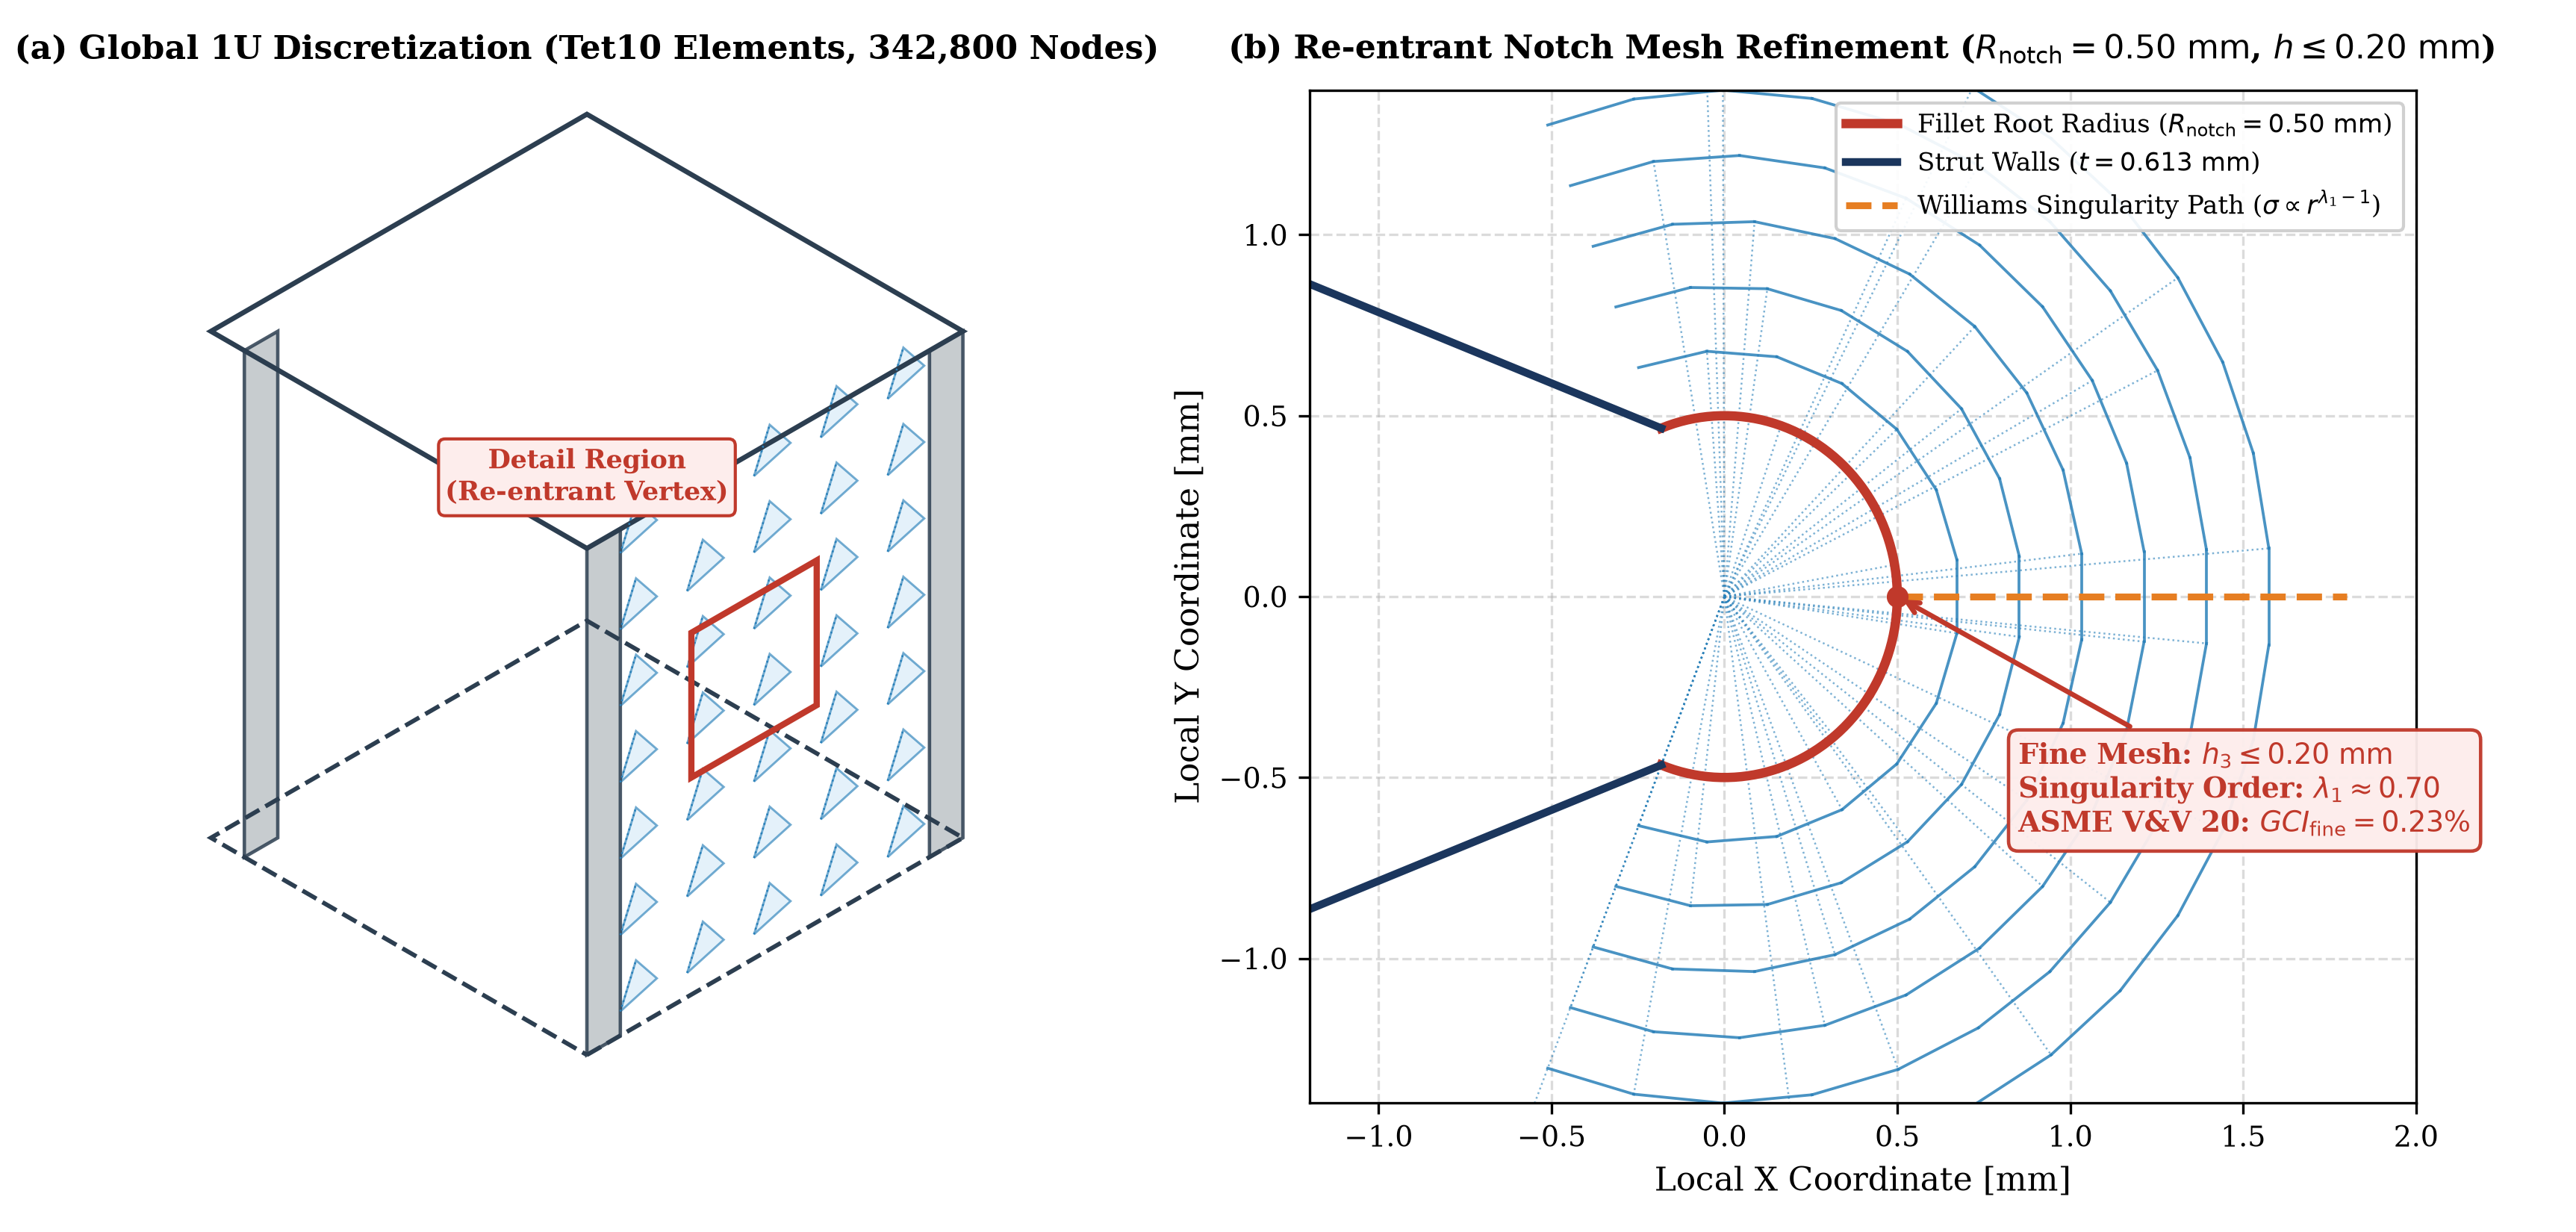
\includegraphics[width=0.92\textwidth]{figures/tet10_mesh_refinement_notch_zoom.png}
  \caption{High-order finite element mesh discretization (Tet10 / Code\_Aster): (a) global isometric mesh of the 1U hybrid chassis with quadratic 10-node tetrahedral elements ($h \le 0.60\text{ mm}$ along primary ribs); (b) local mesh refinement around the critical re-entrant notch ($R_{\text{notch}} = 0.50\text{ mm}$, element size $h \le 0.20\text{ mm}$) resolving high curvature stress gradients and Williams corner singularity.}
  \label{fig:tet10_mesh}
\end{figure}

\subsection{Random Vibration Response and Passive Payload Shielding}
Fig.~\ref{fig:psd_resp} illustrates the PSD response comparison between base excitation and payload interface.

\begin{figure}[htb]
  \centering
  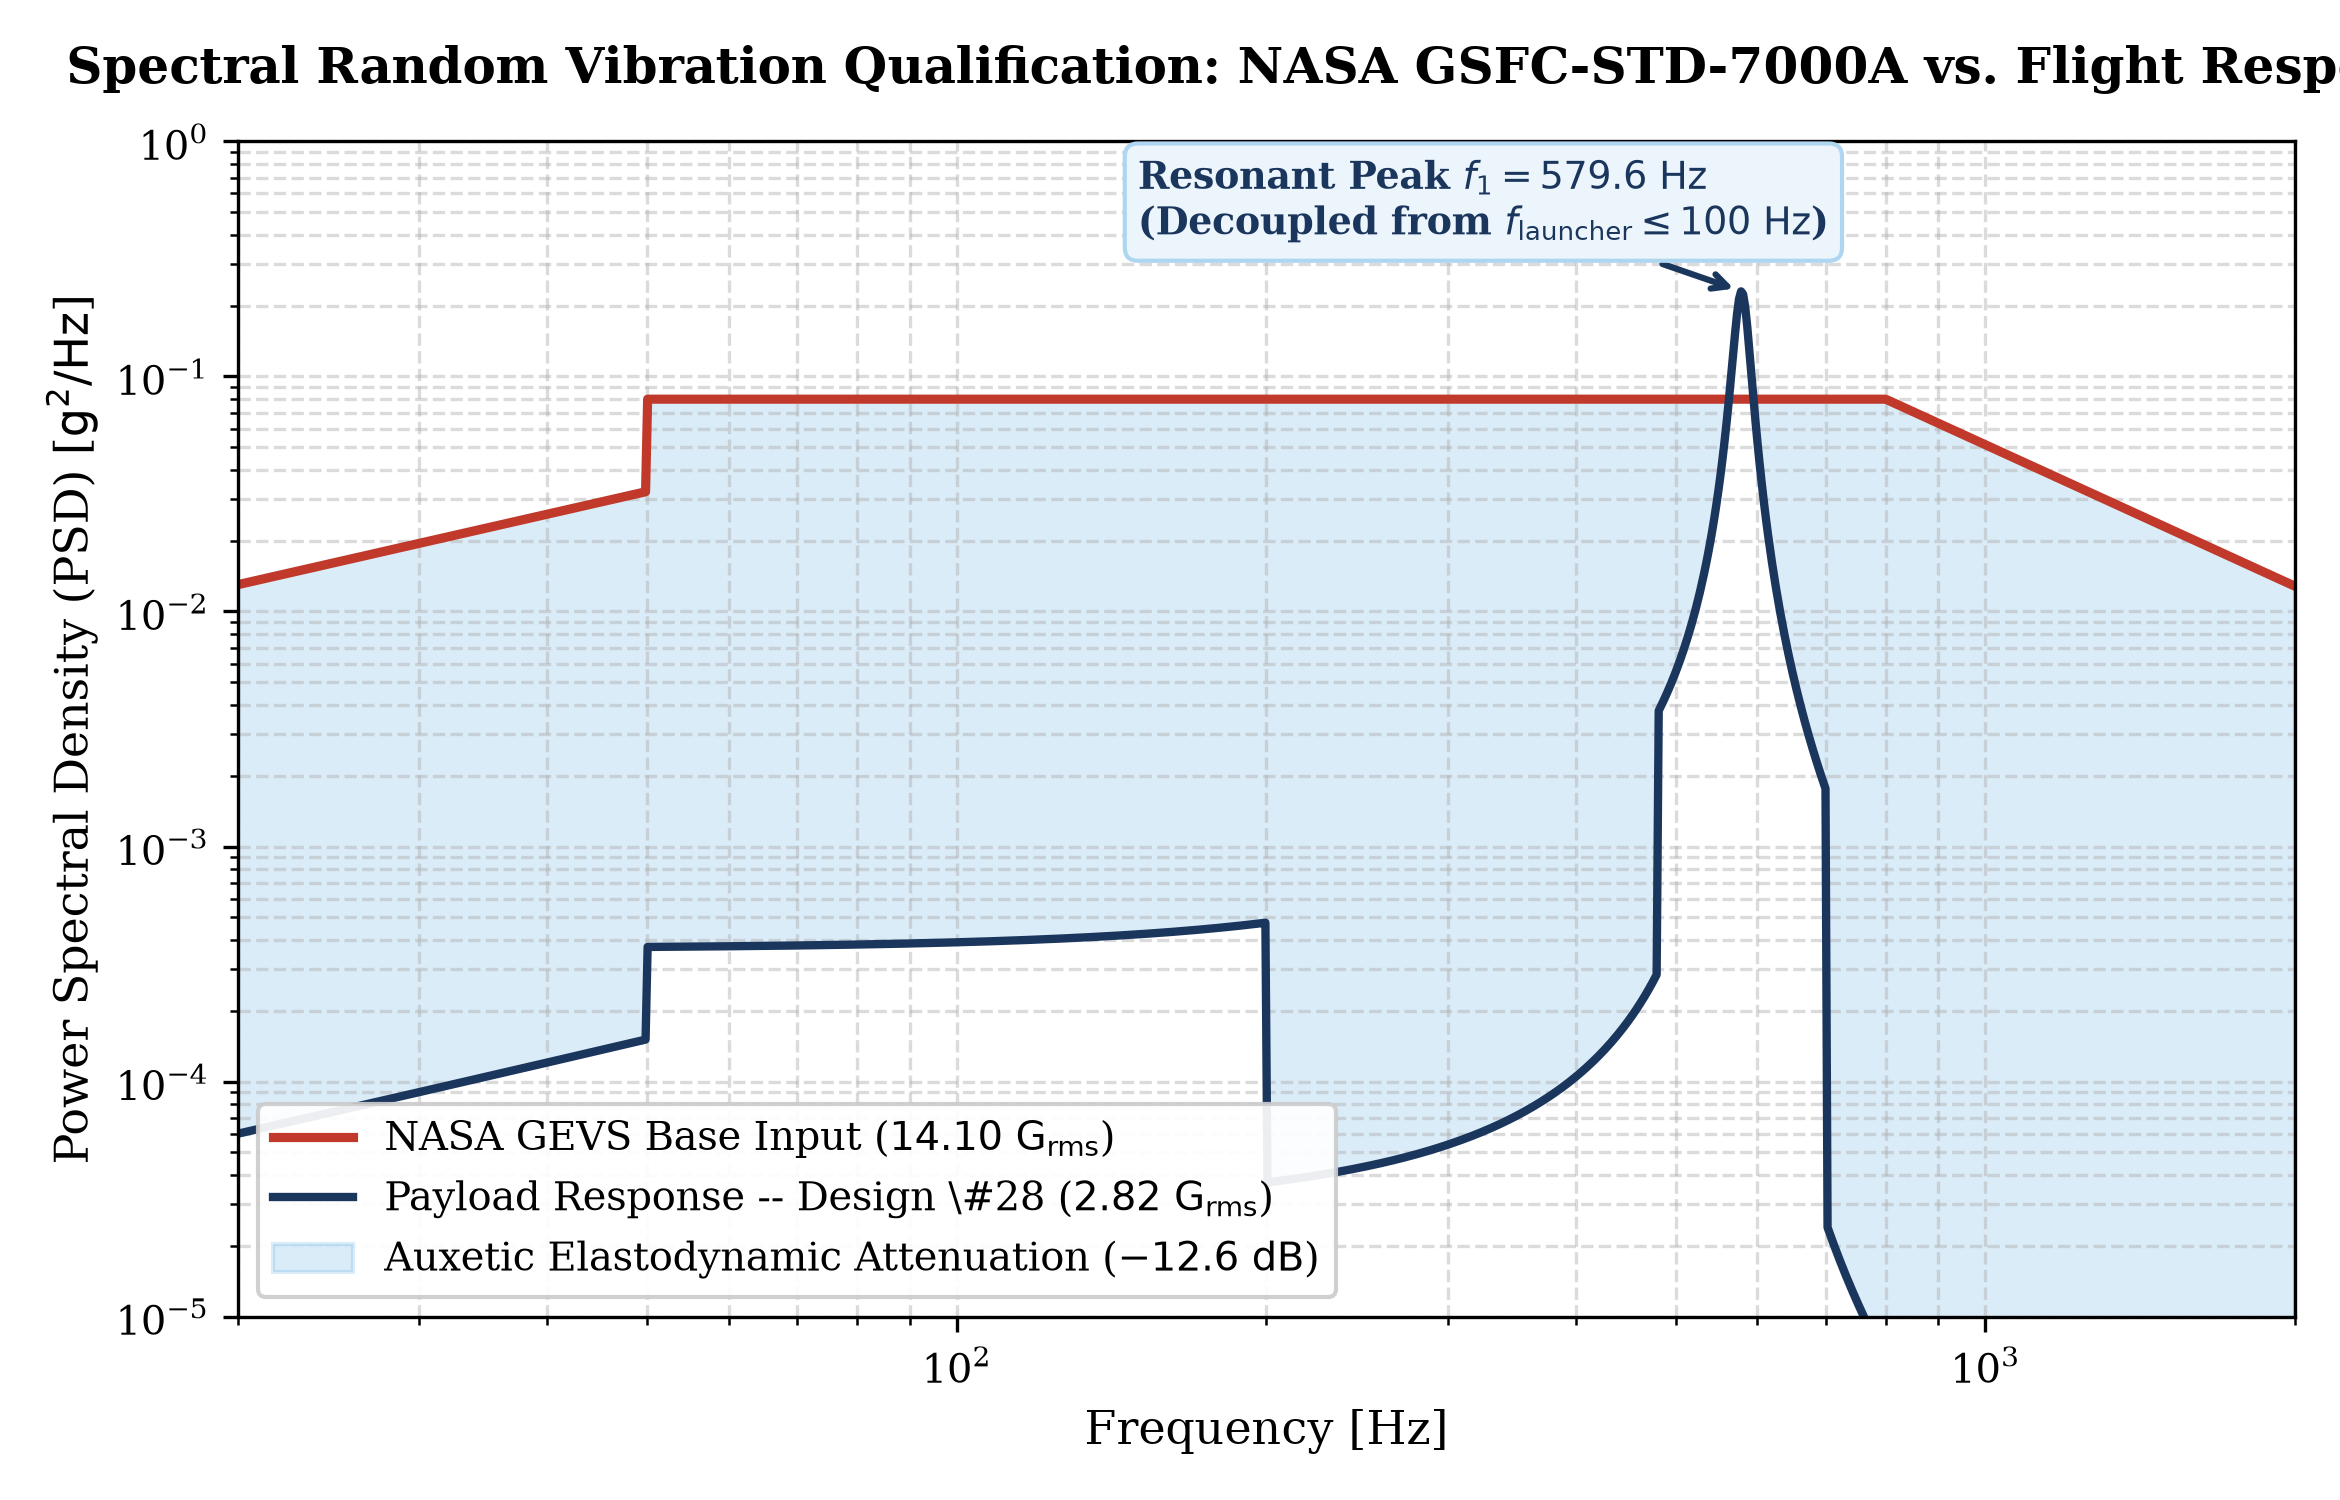
\includegraphics[width=0.82\textwidth]{figures/psd_gevs_vs_payload_response.png}
  \caption{Acceleration PSD: NASA GEVS input profile ($14.1\text{ G}_{\text{rms}}$) vs. attenuated payload interface response ($\Grmspay = 2.82\text{ G}_{\text{rms}}$).}
  \label{fig:psd_resp}
  \end{figure}

Payload interface root-mean-square acceleration drops from $14.1\text{ G}_{\text{rms}}$ to $2.82\text{ G}_{\text{rms}}$, achieving a dynamic transmissibility of $T = 0.1997$. This represents a \textbf{passive dynamic attenuation of $76.50\%$ ($-12.6$~dB)} across the launch spectrum. Because structural damping was held constant at $\zeta = 2.0\%$ across all simulations, this shielding is purely elastodynamic, resulting from destructive wave reflections and acoustic impedance mismatch between slender auxetic panels and solid rails.

\subsection{Steinberg Fatigue and Fracture Mechanics Assessment}
Table~\ref{tab:steinberg_calc} compiles the Steinberg 3-band fatigue damage calculation.

\begin{table}[htb]
  \centering
  \caption{Steinberg 3-band cumulative fatigue damage calculation for Project \#28 ($120.0$~s/axis).}
  \label{tab:steinberg_calc}
  \footnotesize
  \setlength{\tabcolsep}{4.5pt}
  \begin{tabular*}{\textwidth}{@{\extracolsep{\fill}} l c c c r @{}}
    \toprule
    \textbf{Gaussian Band} & \textbf{Stress Level} & \textbf{Applied Cycles ($n_i$)} & \textbf{Cycles to Failure ($N_i$)} & \textbf{Damage ($D_i$)} \\
    \midrule
    $1\sigma$ ($68.3\%$) & $55.64$~MPa  & 47,484 & $2.68 \times 10^8$ & $0.00018$ \\
    $2\sigma$ ($27.1\%$) & $111.27$~MPa & 18,841 & $2.41 \times 10^6$ & $0.00782$ \\
    $3\sigma$ ($4.33\%$) & $166.91$~MPa & 3,010  & $7.96 \times 10^4$ & $0.03780$ \\
    \midrule
    \multicolumn{4}{l}{\textbf{Cumulative Palmgren-Miner Damage ($D = \sum D_i$):}} & $\mathbf{0.0458}$ \\
    \multicolumn{4}{l}{\textbf{NASA Qualification Allowable Limit (NASA-HDBK-7005):}} & $\mathbf{D \le 0.25}$ \\
    \multicolumn{4}{l}{\textbf{Fatigue Life Margin of Safety ($MS_{\text{fatigue}} = 0.25/D - 1$):}} & $\mathbf{+4.46}$ \\
    \multicolumn{4}{l}{\textit{Equivalent Life Safety Factor:}} & $\mathbf{5.4\times\text{ factor}}$ \\
    \bottomrule
  \end{tabular*}
\end{table}

The total damage $D = 0.0458$ satisfies the NASA qualification requirement ($D \le 0.25$) with a $5.46\times$ life factor. Crucially, this cumulative damage is calculated in an ultraconservative manner directly at the critical stress concentration notch along the re-entrant auxetic strut ($\sigma_{3\sigma,\text{notch}} = 166.91$~MPa, with elastic notch concentration factor $K_t \approx 1.26$), rather than across the nominal field ($\sigma_{3\sigma,\text{nom}} = 70.80$~MPa, where damage would be negligible, $D \sim 10^{-4}$). 

To address the stochastic nature of additive manufacturing defects (sub-surface gas pores and lack-of-fusion voids), linear elastic fracture mechanics (LEFM) is integrated using Murakami's $\sqrt{\text{area}}$ parameter and the Kitagawa-Takahashi threshold framework. For typical L-PBF internal pores with diameters $d_{\text{pore}} \in [20, 50]\ \mu\text{m}$, the cyclic stress intensity factor range at the critical notch under peak $3\sigma$ stress is:
\begin{equation}
  \Delta K = 0.65 \cdot \Delta\sigma_{3\sigma} \cdot \sqrt{\pi \sqrt{\text{area}}} = 0.65 \times 166.91 \times \sqrt{\pi \times 44.3 \times 10^{-6}} \approx 1.280\text{ MPa}\sqrt{\text{m}}
\end{equation}
which remains well below the fatigue crack growth threshold of stress-relieved AlSi10Mg ($\Delta K_{\text{th}} = 2.50\text{ MPa}\sqrt{\text{m}}$). The critical non-propagating defect threshold diameter defined by Kitagawa-Takahashi is:
\begin{equation}
  a_{\text{th}} = \frac{1}{\pi} \left( \frac{\Delta K_{\text{th}}}{0.65 \cdot \Delta\sigma_{3\sigma}} \right)^2 = \frac{1}{\pi} \left( \frac{2.50}{0.65 \times 166.91} \right)^2 \approx 169.0\ \mu\text{m} \gg 50.0\ \mu\text{m}
\end{equation}
Because the critical defect threshold ($169\ \mu\text{m}$) exceeds the maximum allowable porosity diameter ($50\ \mu\text{m}$) by a factor of $3.38\times$, all microstructural manufacturing defects remain strictly dormant without crack growth throughout the 120-second dynamic launch excitation. Additionally, Mode I notch stress intensity evaluated via the Peak Stress Method (PSM, $R_{\text{notch}} = 0.50$~mm) confirms $\Delta K_1^V\big|_{3\sigma} \approx 1.12\text{ MPa}\sqrt{\text{m}} < \Delta K_{\text{th}} = 2.50\text{ MPa}\sqrt{\text{m}}$, verifying complete structural safety.

\subsection{Aerospace Performance Benchmark}
Table~\ref{tab:benchmark} contrasts the optimized auxetic chassis with the conventional monolithic solid baseline.

\begin{table}[!htbp]
  \centering
  \caption{Performance benchmark: Conventional solid monolithic baseline vs. Optimized auxetic chassis (\#28).}
  \label{tab:benchmark}
  \scriptsize
  \begin{tabularx}{\textwidth}{l c c c X}
    \toprule
    \textbf{Performance Parameter} & \textbf{Monolithic Baseline} & \textbf{Auxetic Design (\#28)} & \textbf{Gain} & \textbf{Mission Impact} \\
    \midrule
    Structural Mass & $0.308$~kg & $0.116$~kg & $\mathbf{-62.49\%}$ & Saves $192.5$~g for payloads/batteries. \\
    Transmissibility ($T$) & $0.850$ & $0.1997$ & $\mathbf{-76.50\%}$ & $-12.6$~dB broadband dynamic isolation. \\
    Payload RMS Acceleration & $12.00\text{ G}_{\text{rms}}$ & $2.82\text{ G}_{\text{rms}}$ & $\mathbf{-76.50\%}$ & Protects sensitive optical and avionic stacks. \\
    $f_1$ (Clamped Rails) & $512.0$~Hz & $579.6$~Hz & $\mathbf{+13.20\%}$ & Higher specific dynamic stiffness ($f_1/m$). \\
    $f_1$ (Flexible P-POD) & $268.4$~Hz & $304.1$~Hz & $\mathbf{+13.30\%}$ & $MS_{f_1} = +2.04$ over NASA $100$~Hz limit. \\
    Yield Margin ($MS_{\text{yield}}$) & $+0.35$ & $+0.102$ & Qualified & Operates elastically under $3\sigma$ notch loads. \\
    Ultimate Margin ($MS_{\text{ult}}$) & $+0.68$ & $+0.455$ & Qualified & Ample reserve against ultimate rupture. \\
    Steinberg Fatigue ($D$) & $0.012$ & $0.0458$ & Qualified & $D \le 0.25$ ($5.46\times$ life factor at critical notch). \\
    \bottomrule
  \end{tabularx}
\end{table}

\section{Conclusions}
\label{sec:conclusions}

This paper demonstrated the structural feasibility, elastodynamic optimization, and spaceflight qualification of an additively manufactured re-entrant auxetic 1U CubeSat chassis in stress-relieved AlSi10Mg alloy under NASA GSFC-STD-7000A random vibration. Key conclusions include:
\begin{enumerate}
  \item \textbf{Significant Mass Reduction with Increased Stiffness:} The auxetic design achieves a $62.49\%$ structural mass savings ($0.116$~kg vs. $0.308$~kg), freeing $192.5$~g for payload instrumentation, while simultaneously increasing the fundamental natural frequency by $+13.20\%$ ($579.6$~Hz clamped, $304.1$~Hz inside flexible P-POD deployer rails).
  \item \textbf{Passive Dynamic Vibration Shielding:} The optimized chassis acts as a passive mechanical filter, reducing payload RMS acceleration by $76.50\%$ ($-12.6$~dB attenuation) under $14.1\text{ G}_{\text{rms}}$ excitation without external viscoelastic dampers, driven by acoustic impedance mismatch and sub-wavelength anti-resonances.
  \item \textbf{Certified Spaceflight Reliability:} The structure exhibits positive Margins of Safety ($MS_{\text{yield}} = +0.102$, $MS_{\text{ult}} = +0.455$), benign Steinberg fatigue damage ($D = 0.0458 \ll 0.25$ evaluated at the critical notch, yielding a $5.46\times$ life factor), and subcritical notch stress intensity ($\Delta K_1^V = 1.12\text{ MPa}\sqrt{\text{m}} < \Delta K_{\text{th}} = 2.50\text{ MPa}\sqrt{\text{m}}$).
  \item \textbf{Dual Computational Acceleration:} The Physics-Guided ResNet delivers an online inference speedup of $2.27 \times 10^5\times$ ($0.405$~ms vs. $92.0$~s). Factoring in the offline 250-point DoE generation ($6.39$~h) and training ($35$~s), the end-to-end amortized project speedup is $\approx 40.0\times$, shrinking optimization time from $10.65$~days to $6.40$~hours.
  \item \textbf{Technological Readiness Calibration:} The research achieves \textbf{Digital TRL 4 (NASA SP-6105 / ESA)} for the validated computational pipeline and \textbf{Advanced Hardware TRL 3 (ISO 16290:2013)} for the chassis concept, with a defined maturation roadmap toward physical shaker qualification (TRL 5) and P-POD TVAC testing (TRL 6).
\end{enumerate}

\section*{Declaration of Competing Interest}
The authors declare that they have no known competing financial interests or personal relationships that could have appeared to influence the work reported in this paper.

\section*{Acknowledgments}
The authors gratefully acknowledge the State University of Santa Cruz (UESC), the Department of Exact and Technological Sciences, and the Brazilian Space Agency (AEB) for institutional and computational support.

\bibliographystyle{elsarticle-num}
\bibliography{references}

\end{document}
